\documentclass[journal]{IEEEtranTIE}

\usepackage{amsmath,amsfonts}
\usepackage{array}
\usepackage{booktabs}
\usepackage{cite}
\usepackage{graphicx}
\usepackage{microtype}
\usepackage{multirow}
\usepackage{stfloats}
\usepackage{placeins}
\usepackage{xspace}
\usepackage{xurl}
\usepackage[hidelinks]{hyperref}
\usepackage{etoolbox}
\graphicspath{{figures/}}

\newcommand{\model}{MCGI-YOLO\xspace}
\newcolumntype{L}[1]{>{\raggedright\arraybackslash}p{#1}}

% Keep the journal fonts and margins; tighten only float and biography spacing.
\setlength{\textfloatsep}{12pt plus 2pt minus 2pt}
\setlength{\dbltextfloatsep}{12pt plus 2pt minus 2pt}
\setlength{\floatsep}{10pt plus 2pt minus 2pt}
\setlength{\dblfloatsep}{10pt plus 2pt minus 2pt}
\makeatletter
\renewcommand{\@IEEEBIOskipN}{1\baselineskip}
\makeatother

\begin{document}
\raggedbottom

\title{An Edge System and MCGI-YOLO for Fabric Defect Detection and Closed-Loop Control in Circular Knitting Machines}

\author{Kangzhao Tan\textsuperscript{\#}, Jiarui Zhang\textsuperscript{\#}, Junjie Yu, Heng Wu, Jing Lin\textsuperscript{*}, and Chunhua He\textsuperscript{*}%
\thanks{Manuscript received October 22, 2026. (\textsuperscript{\#}These authors contributed equally: Kangzhao Tan, Jiarui Zhang) (\textsuperscript{*}Corresponding authors: Jing Lin and Chunhua He).}%
\thanks{\begingroup\urlstyle{same}Kangzhao Tan, Jiarui Zhang, Junjie Yu, and Chunhua He are with the School of Computer Science, Guangdong University of Technology, Guangzhou 510006, China (e-mail: \protect\url{tankangzhao@mails.gdut.edu.cn}; \protect\url{zhangjiarui1@mails.gdut.edu.cn}; \protect\url{yujunjie2@mails.gdut.edu.cn}; \protect\url{hechunhua@pku.edu.cn}). Heng Wu is with the School of Automation, Guangdong University of Technology, Guangzhou 510006, China (e-mail: \protect\url{heng.wu@gdut.edu.cn}). Jing Lin is with the Classroom Management Center, Guangdong University of Technology, Guangzhou 510006, China (e-mail: \protect\url{lj@gdut.edu.cn}).\endgroup}%
}

\maketitle

\begin{abstract}
Defect detection is critical for circular knitting production, where persistent needle or yarn abnormalities lead to repeated fabric defects, resulting in severe material waste and economic losses. Existing methods are rarely tailored to circular knitting machines and tend to be cost-prohibitive, limiting large-scale industrial deployment. To address this issue, we present a low-cost, dedicated defect detection and closed-loop control system for circular knitting machines, which triggers image acquisition from machine rotation, halts the machine upon defect detection to interrupt defect propagation, and alerts the operator for corrective intervention, forming a complete production–detection–control loop. To further improve detection accuracy for diverse fabric defect morphologies and scales, we propose a lightweight detector termed \model. To model the morphological continuity of elongated defects, morphology-aware context encoding (MCE) augments backbone features with spatially extended context. To accommodate variations in defect morphology and scale, gated interpolation upsampling (GIU) adapts the reconstruction of higher-level context before fusion with local features, using a compact content-adaptive gate. On a real-world dataset collected from a circular-knitting production line, \model achieves 97.2\% mAP50 and 65.5\% mAP50--95, improving on the YOLOv8n baseline by 6.7 and 7.1 percentage points, respectively. After INT8 conversion, the model reaches an inference throughput of 22 FPS on the edge device. The proposed system provides a cost-effective solution for real-time defect detection in circular-knitting production.
\end{abstract}

\begin{IEEEkeywords}
Circular knitting machine, fabric defect detection, edge computing, morphology-aware context encoding(MCE), gated interpolation upsampling(GIU), YOLO.
\end{IEEEkeywords}

\markboth{IEEE TRANSACTIONS ON INDUSTRIAL ELECTRONICS}{}

\section{Introduction}
\IEEEPARstart{C}{ircular} knitting machines are key production equipment for high-volume weft-knit fabric, which is widely used in everyday clothing such as T-shirts and sportswear \cite{cottonworksKnitBasics,woolmarkCircularKnitting,cottonworksSingleDouble}. The International Textile Manufacturers Federation reported approximately 24,500 global shipments of circular knitting machines in 2025 \cite{itmf2025press}. Globally, approximately 92 million tonnes of textile waste are generated annually, highlighting the importance of reducing avoidable material losses \cite{unep2025textilewaste}. Conventional quality checks are often performed after knitting is completed. A persistent needle or yarn abnormality can therefore generate repeated defects along the fabric before discovery, accumulating substantial fabric waste and economic losses \cite{takeuchi2018knitted,akter2022material,xiang2023hooknet}. To prevent such losses, real-time detection during knitting is needed to identify these defects early and enable timely intervention before further defective fabric is produced.

Edge computing offers a practical pathway toward such real-time detection, and has been increasingly adopted for industrial defect detection. In textile applications, Machado et al. deployed YOLO11n on a Jetson Orin Nano to detect solid-color cotton and linen fabrics on a fabric rolling line \cite{machado2025edgefabric}. Yan et al. deployed an improved YOLOv5s model on a Huawei Ascend 310-based Atlas platform to detect warp-knitted lace on warp-knitting machines \cite{yan2026warplace}. Beyond textile detection, Wang et al. and Zhang et al. deployed an improved YOLOv5s model for rail surface defect detection and an improved Faster R-CNN detector with convolutional feature reuse for UAV-based insulator defect detection, respectively, both on Jetson Xavier NX \cite{wang2024rail,zhang2026uavedge}. Li et al. deployed LiteYOLO-ID on a Jetson TX2 NX for insulator defect detection \cite{li2024liteyolo}, and Zhao et al. implemented KAM-Net on a Xilinx ZCU102 FPGA for glass defect segmentation \cite{zhao2025kamnet}. These studies collectively demonstrate the applicability of edge computing to industrial defect detection in their respective scenarios. However, such platforms are not tailored to the sensing, control, and installation constraints of circular knitting machines. The relatively high cost of general-purpose computing platforms, together with the additional integration effort required for image acquisition and machine control, hinders economically viable deployment across large numbers of machines.

In terms of detection algorithms, YOLO-based detectors have been widely explored for industrial defect detection because of their efficient inference and explicit defect localization \cite{redmon2016yolo}. FA-YOLO combines receptive-field enhancement, attention, and adaptive spatial feature fusion \cite{yu2024fayolo}. DGHR-YOLO integrates deformable convolution for morphology adaptation with a high-level screening feature pyramid and lightweight feature processing \cite{zhang2025dghr}. Zhao et al. proposed attention-based multiscale feature fusion (AMFF), combining intralayer feature enhancement and cross-layer attention to strengthen weak defect representations on fabric and aluminum surfaces \cite{zhao2024amff}. An and Wan introduced JDCBL, combining contextual Transformer features with balanced contrastive learning to address scale variation and long-tailed defect categories in fabric detection \cite{an2025jdcbl}. Wang et al. developed RRNet, a lightweight rotated fabric defect detector that combines position-guided fusion and multiscale rotation-guided strip coupling to model elongated and tilted defect structures \cite{wang2026rrnet}. Together, these methods advance the representation of subtle defects, irregular shapes, and scale variation. Related work on photovoltaic-cell and pipeline-weld detection also explores task-specific feature pyramids, contextual relations, and lightweight rotated representations \cite{su2022baf,shen2024crnet,liu2025lrnet}. However, these methods are tailored to their respective detection targets and may not be directly applicable to defect detection on circular knitting machines. Defects on circular knitting machines exhibit diverse morphologies and scales, ranging from horizontal and vertical elongated patterns to localized holes. In addition, modules such as deformable convolution and attention often introduce substantial computational overhead, making them less suitable for deployment on resource-constrained edge devices.

Motivated by these limitations, we design and implement a low-cost, dedicated defect detection and closed-loop control system for circular knitting machines. The system integrates a power adapter, a global-shutter camera with LED illumination, a coaxial serializer/deserializer (SerDes) image-transmission link, a Hall sensor, and a self-developed edge device. For defect detection within this system, we develop \model, a lightweight detector that incorporates morphology-aware and scale-aware design for fabric defects. MCE supplies spatially extended morphology-aware context for horizontal and vertical elongated defects. GIU addresses the differing reconstruction needs of elongated defects and holes of varying sizes by adaptively adjusting the interpolation of higher-level context. Together, the two components connect morphology-aware context encoding with spatial reconstruction within a compact parameter budget.

The main contributions of our work are as follows.
\begin{enumerate}
  \renewcommand{\labelenumi}{(\arabic{enumi})}
  \item We design and implement a dedicated defect detection and closed-loop system for circular knitting machines, integrating image acquisition, camera transmission, edge inference, and local machine-stop control, and demonstrate its deployment on a real production line.
  \item We develop MCE to explicitly incorporate the morphology priors of horizontal and vertical elongated defects. It embeds spatially extended, morphology-aware context in a partial C2f branch with small additional overhead.
  \item We design GIU to accommodate the diverse morphologies and scales of circular-knitting defects, including elongated defects and holes of varying sizes. A compact spatial gate adapts a convex combination of two fixed interpolation paths, balancing response replication and neighborhood smoothing in the top-down path.
\end{enumerate}

The remainder of this paper is organized as follows. Section~\ref{sec:system-design} presents the defect detection and closed-loop control system. Section~\ref{sec:method} describes MCGI-YOLO and its two components. Section~\ref{sec:experimental-setup} defines the dataset and evaluation protocol. Section~\ref{sec:results} reports detector comparisons, component ablation, and model deployment. Section~\ref{sec:conclusion} concludes the paper.

\section{Defect Detection and Closed-Loop Control System}
\label{sec:system-design}
\subsection{System Overview}
\label{sec:system-overview}
We design and implement a dedicated defect detection and closed-loop control system for circular knitting machines, as shown in Fig.~\ref{fig:interactions}. The closed-loop workflow begins when the operator starts the machine. The Hall sensor detects machine rotation and triggers the edge device to activate the camera and LED illumination for image acquisition and defect detection. When a defect is detected, the edge device immediately sends a stop command to the machine controller to prevent further defect propagation, uploads the defect image and record to the cloud, and pushes an alert notification to the operator. After the operator inspects the reported defect, resolves the production fault, and restarts the machine, the rotation signal reactivates detection. This sequence forms a complete production–detection–control loop. The system is organized into three functional subsystems: power supply, image acquisition and transmission, and processor. The following subsections describe their designs and hardware implementation.

\begin{figure*}[!tbp]
\centering
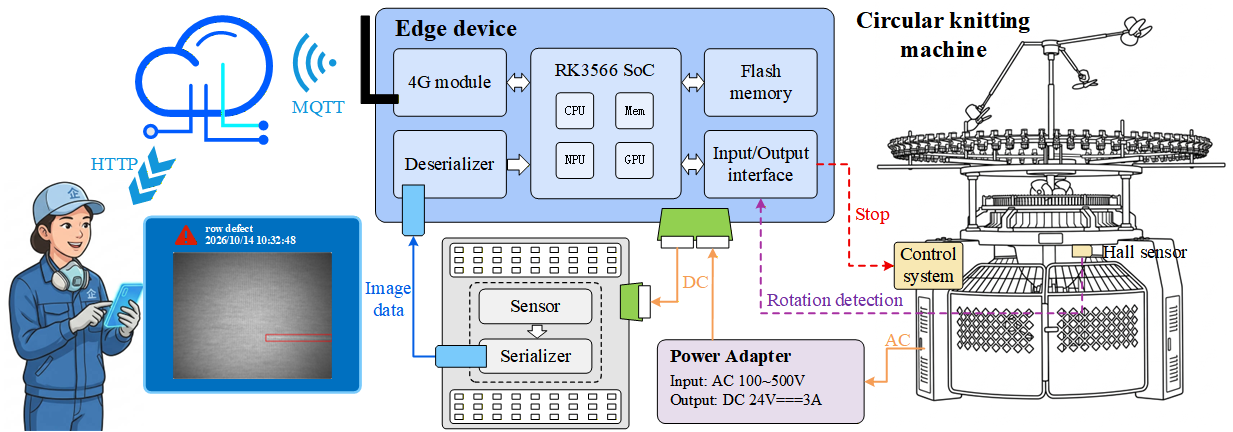
\includegraphics[width=0.92\textwidth]{system.png}
\caption{The device comprises LED illumination control, a coaxial image link to the RK3566, 4G cloud connectivity, and I/O for rotation sensing and machine control.}
\label{fig:interactions}
\end{figure*}

\subsection{Power Supply Subsystem}
To accommodate different industrial supply voltages across countries and regions, we design a power adapter with a 100--500 V AC input range and a 24 V DC output rated at 3 A. The adapter first supplies this output to the device. The device then supplies the LED illumination. By adjusting the current delivered to the LEDs, the device controls the illumination brightness to suit the image-acquisition conditions. This arrangement integrates LED power delivery and brightness control into the device.

\subsection{Image Acquisition and Transmission Subsystem}
The rapid rotation of circular knitting machines requires imaging that preserves defect geometry and fine spatial detail. We therefore select a SmartSens SC130GS global-shutter sensor (SmartSens Technology Co., Ltd., Shanghai, China) at $1280\times1024$ resolution, which exposes all pixels simultaneously to avoid motion-induced distortion from sequential row exposure. At a camera-to-fabric distance of approximately 10 cm, the field of view is approximately $16\times12$ cm, with the 16 cm dimension aligned with the horizontal direction of fabric motion.

Factory machinery creates an electromagnetically noisy environment, and installation requires the camera and edge device to be separated by a cable run. We therefore use serializer/deserializer (SerDes) transmission over shielded coaxial cable to accommodate remote camera placement and the interference environment. Specifically, the THCV241A serializer and THCV242A deserializer (THine Electronics, Inc., Tokyo, Japan) bridge the camera-side and processor-side MIPI CSI-2 interfaces. The link supports a maximum serial line rate of 4.0 Gb/s per lane, corresponding to a rated effective rate of 3.2 Gb/s \cite{thineTHCV241A,thineTHCV242A}.

The camera is configured to transmit $1280\times1024$ RAW10 images at 30 frames/s. With $b=10$ bits per pixel, the active-image payload rate is
\begin{equation}
\begin{aligned}
R_{\mathrm{img}} &= W H b f_{\mathrm{cam}} \\
&=1280\times1024\times10\times30 \\
&=393.216\ \mathrm{Mb/s},
\end{aligned}
\label{eq:serdes-bandwidth}
\end{equation}
where $W$ and $H$ denote the image width and height, and $f_{\mathrm{cam}}$ is the camera acquisition rate. This corresponds to only 12.3\% of the rated single-lane effective capacity, providing a stable image input for the detection system.

\subsection{Processor Subsystem}
\label{sec:coverage}
The processor is selected according to the detection rate required by fabric motion and the camera field of view. Taking a typical circular knitting machine as an example, with a machine diameter of 40 in ($D=1.016$ m) and a rotation period of $T=2$ s, the fabric travels approximately $\pi D=3.192$ m per revolution. With an effective field-of-view width of $w=0.16$ m along the direction of motion, the required frame rate is
\begin{equation}
f_{\min}=\frac{\pi D}{Tw}
=\frac{\pi\times1.016}{2\times0.16}
\approx9.97\ \mathrm{frames/s}.
\label{eq:coverage-rate}
\end{equation}
We set the effective detection-throughput requirement to 10 frames/s. For this throughput target, we select the Rockchip RK3566 (Rockchip Electronics Co., Ltd., Fuzhou, China) to balance processing capability, camera connectivity, and hardware cost. It integrates a quad-core Cortex-A55 CPU and an NPU rated at 1 TOPS for INT8 operations \cite{rockchiprk3566}.

Table~\ref{tab:hardware-platforms} summarizes the hardware specifications of platforms used in related defect detection studies. While high-performance platforms like the NVIDIA Jetson Orin Nano and Xilinx ZCU102 offer substantial computational power, their costs range from hundreds to over 3,000 USD, which can be prohibitive for large-scale deployment. In contrast, our self-developed RK3566 device provides a cost-effective hardware basis for the proposed system at a hardware cost of 60 USD, offering a significant cost advantage over comparable industrial platforms and making it highly suitable for large-scale deployment in textile factories.

\begin{table}[!tbp]
\caption{Hardware platforms used in related defect detection studies.}
\label{tab:hardware-platforms}
\centering
\footnotesize
\setlength{\tabcolsep}{3pt}
\renewcommand{\arraystretch}{1.0}
\begin{tabular}{@{}L{0.45\columnwidth}L{0.33\columnwidth}L{\dimexpr0.22\columnwidth-12pt\relax}@{}}
\toprule
Platform & Compute capability & Price (USD) \\
\midrule
NVIDIA Jetson TX2 NX\cite{li2024liteyolo} & 1.33 TFLOPS (FP16) & 249 \\
NVIDIA Jetson Xavier NX\cite{wang2024rail,zhang2026uavedge} & 21 TOPS (INT8) & 399 \\
NVIDIA Jetson Orin Nano\cite{machado2025edgefabric} & 40 TOPS (INT8) & 499 \\
Huawei Ascend 310\cite{yan2026warplace} & 16 TOPS (INT8) & 550 \\
AMD Xilinx ZCU102\cite{zhao2025kamnet} & 3.45 TOPS (INT8)\textsuperscript{\textdagger} & 3234 \\
Self-developed RK3566 device (Ours) & 1 TOPS (INT8) & 60 \\
\bottomrule
\end{tabular}
\par\vspace{1pt}
\begin{minipage}{\columnwidth}
\footnotesize
\textsuperscript{\textdagger}AMD reference INT8 peak for three B4096 DPU cores.
\end{minipage}
\renewcommand{\arraystretch}{1.0}
\end{table}

\subsection{Hardware Implementation}
\label{sec:hardware-implementation}
Based on the design requirements of the subsystems described above, we develop the corresponding hardware shown in Fig.~\ref{fig:hardware}. The camera assembly (a) combines the image sensor and LED illumination. We design a camera-side interface board (b) that integrates the serializer and coaxial connector, and a mainboard (c) built around the RK3566. The mainboard integrates flash storage, the camera deserializer and coaxial connector, a 4G module with SIM-card and antenna interface, input/output interface, and power-management circuitry. This board-level integration brings image reception, local inference, network communication, machine control, and illumination control into a dedicated edge device. Fig.~\ref{fig:system} shows the system installed on a circular knitting machine in a real production line.

\begin{figure*}[!tbp]
\centering
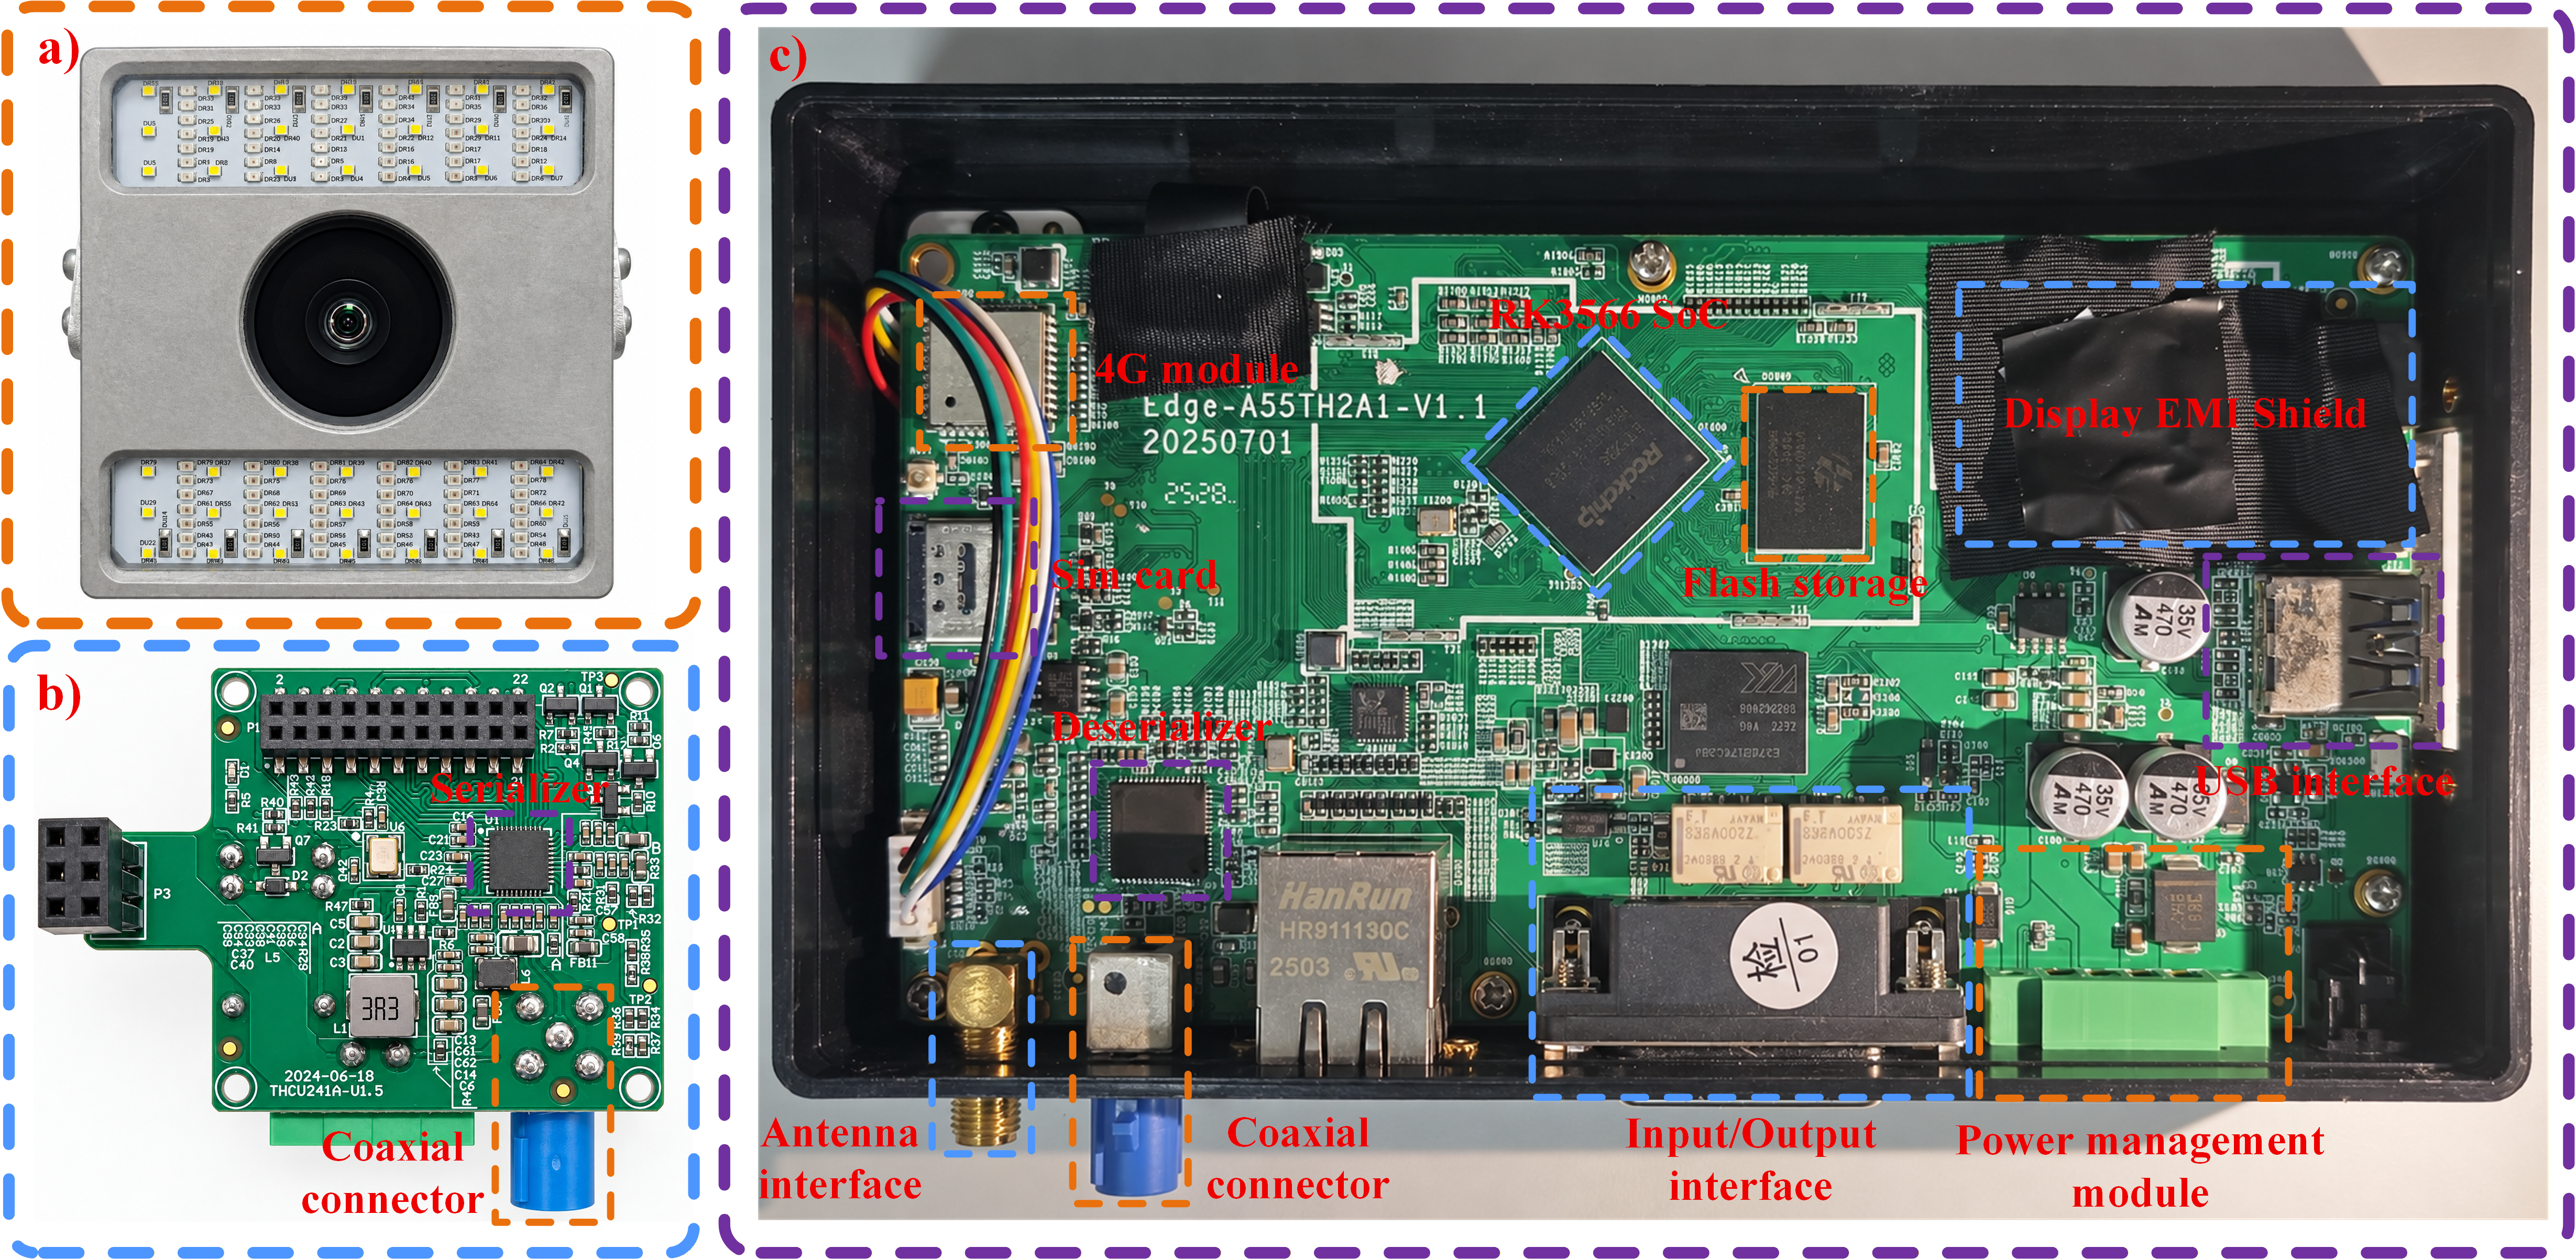
\includegraphics[width=0.86\textwidth]{hardware.png}
\caption{Hardware of the defect detection system: (a) industrial camera with LED illumination; (b) camera-side interface board with a serializer and coaxial connector; and (c) RK3566 edge board with the 4G communication, flash storage, camera-interface, input/output interface, and power-management components.}
\label{fig:hardware}
\end{figure*}

\begin{figure*}[!tbp]
\centering
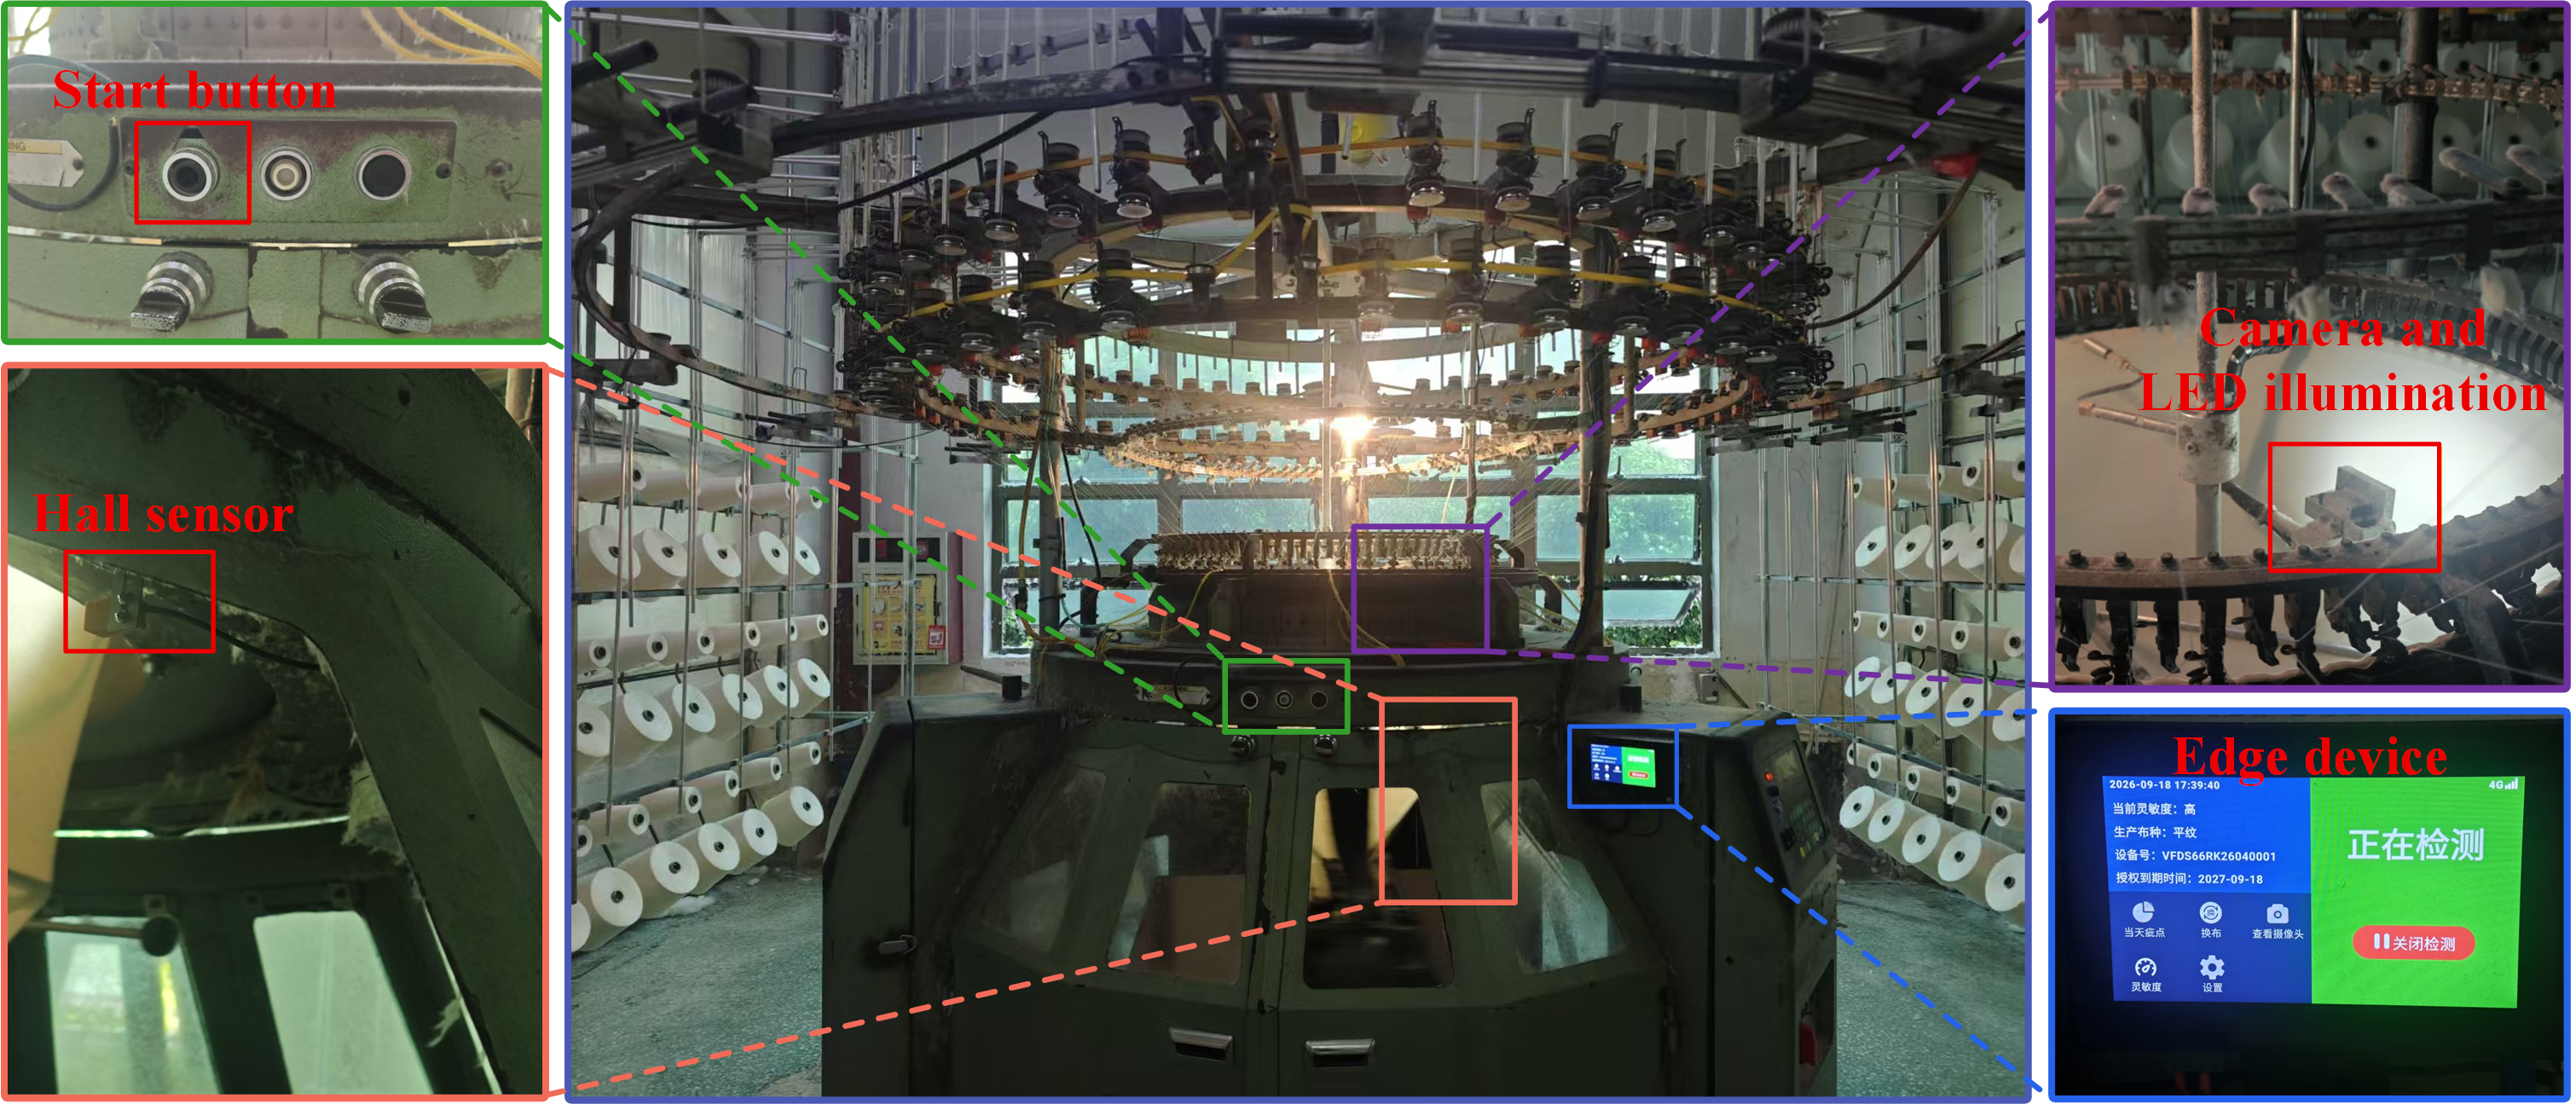
\includegraphics[width=0.86\textwidth]{site.png}
\caption{Actual deployment on the circular knitting machine. The insets highlight the start button, Hall sensor, industrial camera, and RK3566 edge device, respectively.}
\label{fig:system}
\end{figure*}

\section{Detection Algorithm}
\label{sec:method}
\subsection{MCGI-YOLO Architecture}
Fig.~\ref{fig:network} shows \model based on YOLOv8n \cite{ultralytics2023}. Morphology-aware context encoding (MCE) is embedded in the P3 and P4 backbone C2f blocks to capture the continuity of horizontal and vertical elongated defects through spatially extended context. Gated interpolation upsampling (GIU) replaces the two top-down upsampling operations, adapting higher-level context reconstruction to different defect morphologies and scales before lateral feature fusion. The remaining backbone, bottom-up path, and detection head are retained \cite{lin2017fpn,liu2018panet}.

\begin{figure*}[!tbp]
\centering
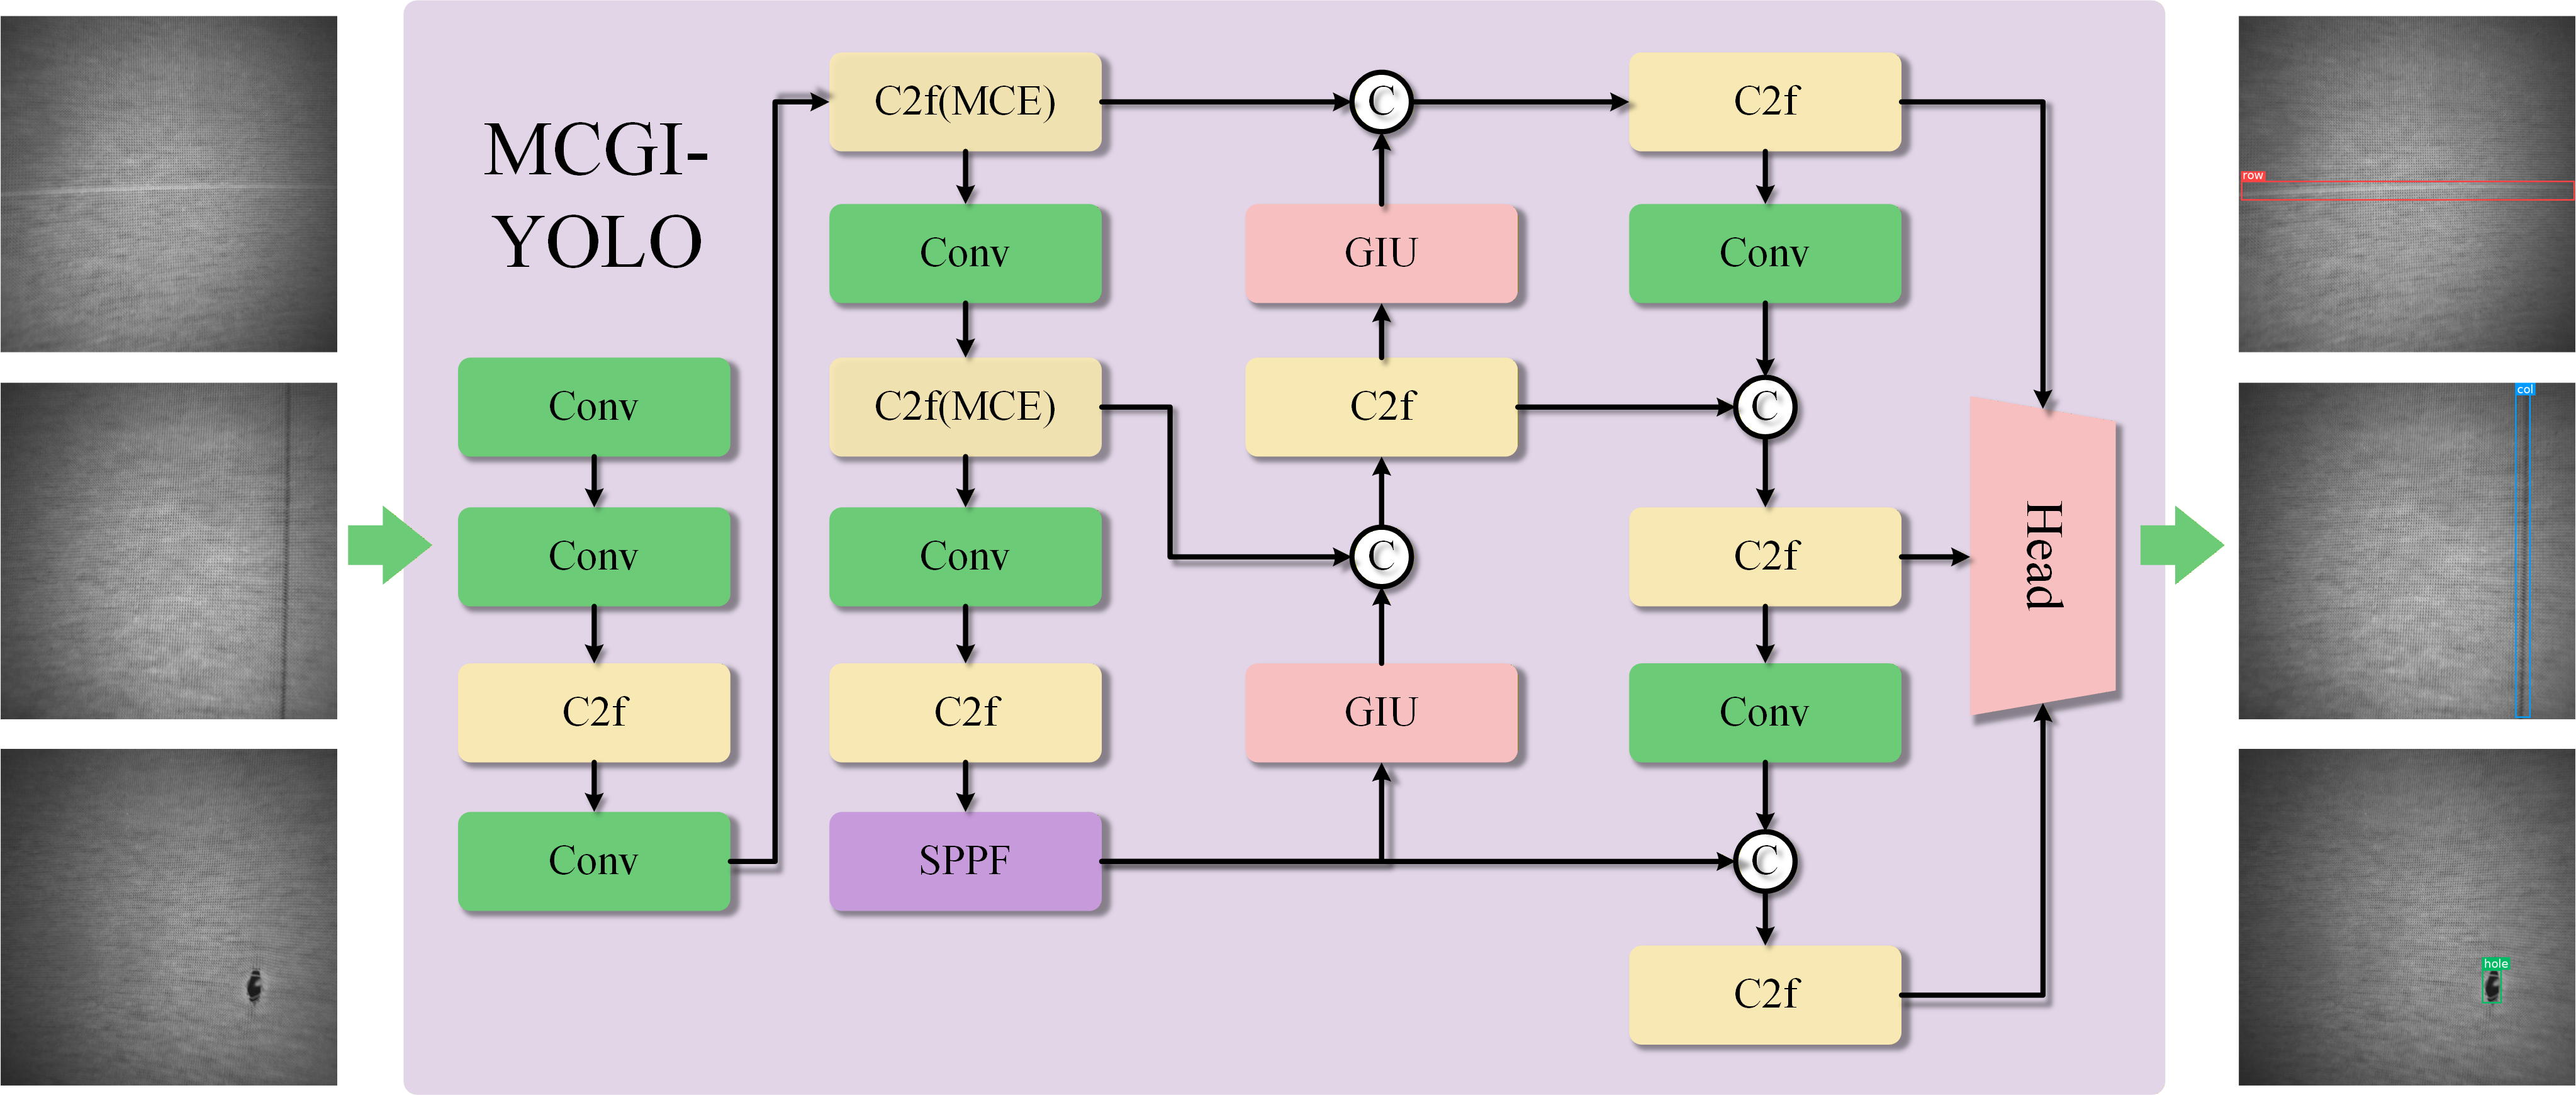
\includegraphics[width=0.9\textwidth]{MCGI-YOLO.png}
\caption{Architecture of \model. MCE operates within the stride-8 and stride-16 backbone C2f stages. GIU replaces the two top-down upsampling operations. The local bottlenecks, bottom-up aggregation path, and three-scale detection head are retained from YOLOv8n.}
\label{fig:network}
\end{figure*}

\subsection{Morphology-Aware Context Encoding}
MCE focuses on horizontal and vertical elongated defects produced by circular knitting machines. Elongated defects are characterized by a high aspect ratio. Their continuity spans across large spatial regions, making it difficult for local receptive fields to establish long-range dependencies. Local feature extraction alone fails to explicitly associate these spatially separated responses as parts of the same defect. Meanwhile, modeling long-range dependencies through dense channel-wise interactions would introduce substantial redundancy, imposing an impractical computational overhead on the RK3566. We therefore develop MCE to incorporate the morphology prior of elongated defects through spatially extended context within a compact computational budget. MCE is inserted after the last bottleneck in the selected C2f blocks, before branch concatenation and fusion [Fig.~\ref{fig:modules}(a)].

\emph{1) Channel Allocation:}
 As illustrated in Fig.~\ref{fig:modules}(d), its input is $F\in\mathbb{R}^{B\times C\times H\times W}$. The channels are divided into two groups: one quarter of the channels, denoted by $U$, are used for morphology-aware context aggregation and residual modulation; the remaining three quarters, denoted by $V$, pass through unchanged. This design intentionally applies morphology-aware context aggregation to only a small channel subset, keeping the computational overhead compact. The two groups are concatenated after modulation, allowing the subsequent fusion to combine morphology-aware and unmodulated features with minimal performance loss. With $q=C/4$, the two groups have sizes $U\in\mathbb{R}^{B\times q\times H\times W}$ and $V\in\mathbb{R}^{B\times(C-q)\times H\times W}$. The split is performed along the channel dimension, preserving the batch and spatial dimensions.

\emph{2) Morphology-Aware Context Aggregation:}
The one-quarter-channel group $U$ feeds the two pooling paths. Here, $b$, $a$, $h$, and $w$ index the batch sample, channel, row, and column, respectively. Inspired by the pooling design of coordinate attention \cite{hou2021coordinate}, we average independently for each sample and channel:
\begin{align}
R_h(b,a,h,1) &= \frac{1}{W}\sum_{w=1}^{W}U(b,a,h,w), \label{eq:pac-row}\\
R_w(b,a,1,w) &= \frac{1}{H}\sum_{h=1}^{H}U(b,a,h,w). \label{eq:pac-column}
\end{align}
Averaging over $W$ aggregates long-range evidence along each row while retaining row positions; averaging over $H$ aggregates long-range evidence along each column while retaining column positions. The resulting descriptors have sizes $B\times q\times H\times1$ and $B\times q\times1\times W$, where the dimension of size 1 corresponds to the spatial direction that was pooled. They pass through $3\times1$ and $1\times3$ depthwise convolutions and are added by broadcasting:
\begin{equation}
T=\operatorname{DW}_{3\times1}(R_h)
 +\operatorname{DW}_{1\times3}(R_w).
\label{eq:pac-context}
\end{equation}
Pooling along full rows and columns provides long-range context, while the $3\times$1 and  $1\times$3 convolutions supplement local information between neighboring positions on the compressed descriptors.

\emph{3) Residual Context Modulation:}
The combined context $T$ is mapped by Hardsigmoid and centered to construct a scaled residual correction:
\begin{align}
G &= \operatorname{HS}(T), \label{eq:pac-map}\\
U' &= U+\gamma\odot U\odot(2G-1), \label{eq:pac-modulation}
\end{align}
where $\operatorname{HS}$ is Hardsigmoid, $\odot$ denotes element-wise multiplication with broadcasting, and $\gamma\in\mathbb{R}^{1\times q\times1\times1}$ is a learnable channel-wise parameter. The context response $G\in[0,1]^{B\times q\times H\times W}$ is centered by $2G-1$ to provide signed modulation, with $\gamma$ controlling its channel-wise strength. The original $U$ is retained through the residual connection, and the corrected one-quarter-channel group $U'$ is concatenated with the unchanged three-quarter-channel group $V$. The corrected group has size $U'\in\mathbb{R}^{B\times q\times H\times W}$, and channel concatenation produces a $B\times C\times H\times W$ output before the original C2f fusion. Zero-initializing $\gamma$ makes the module an identity mapping at initialization.

\begin{figure*}[!tbp]
\centering
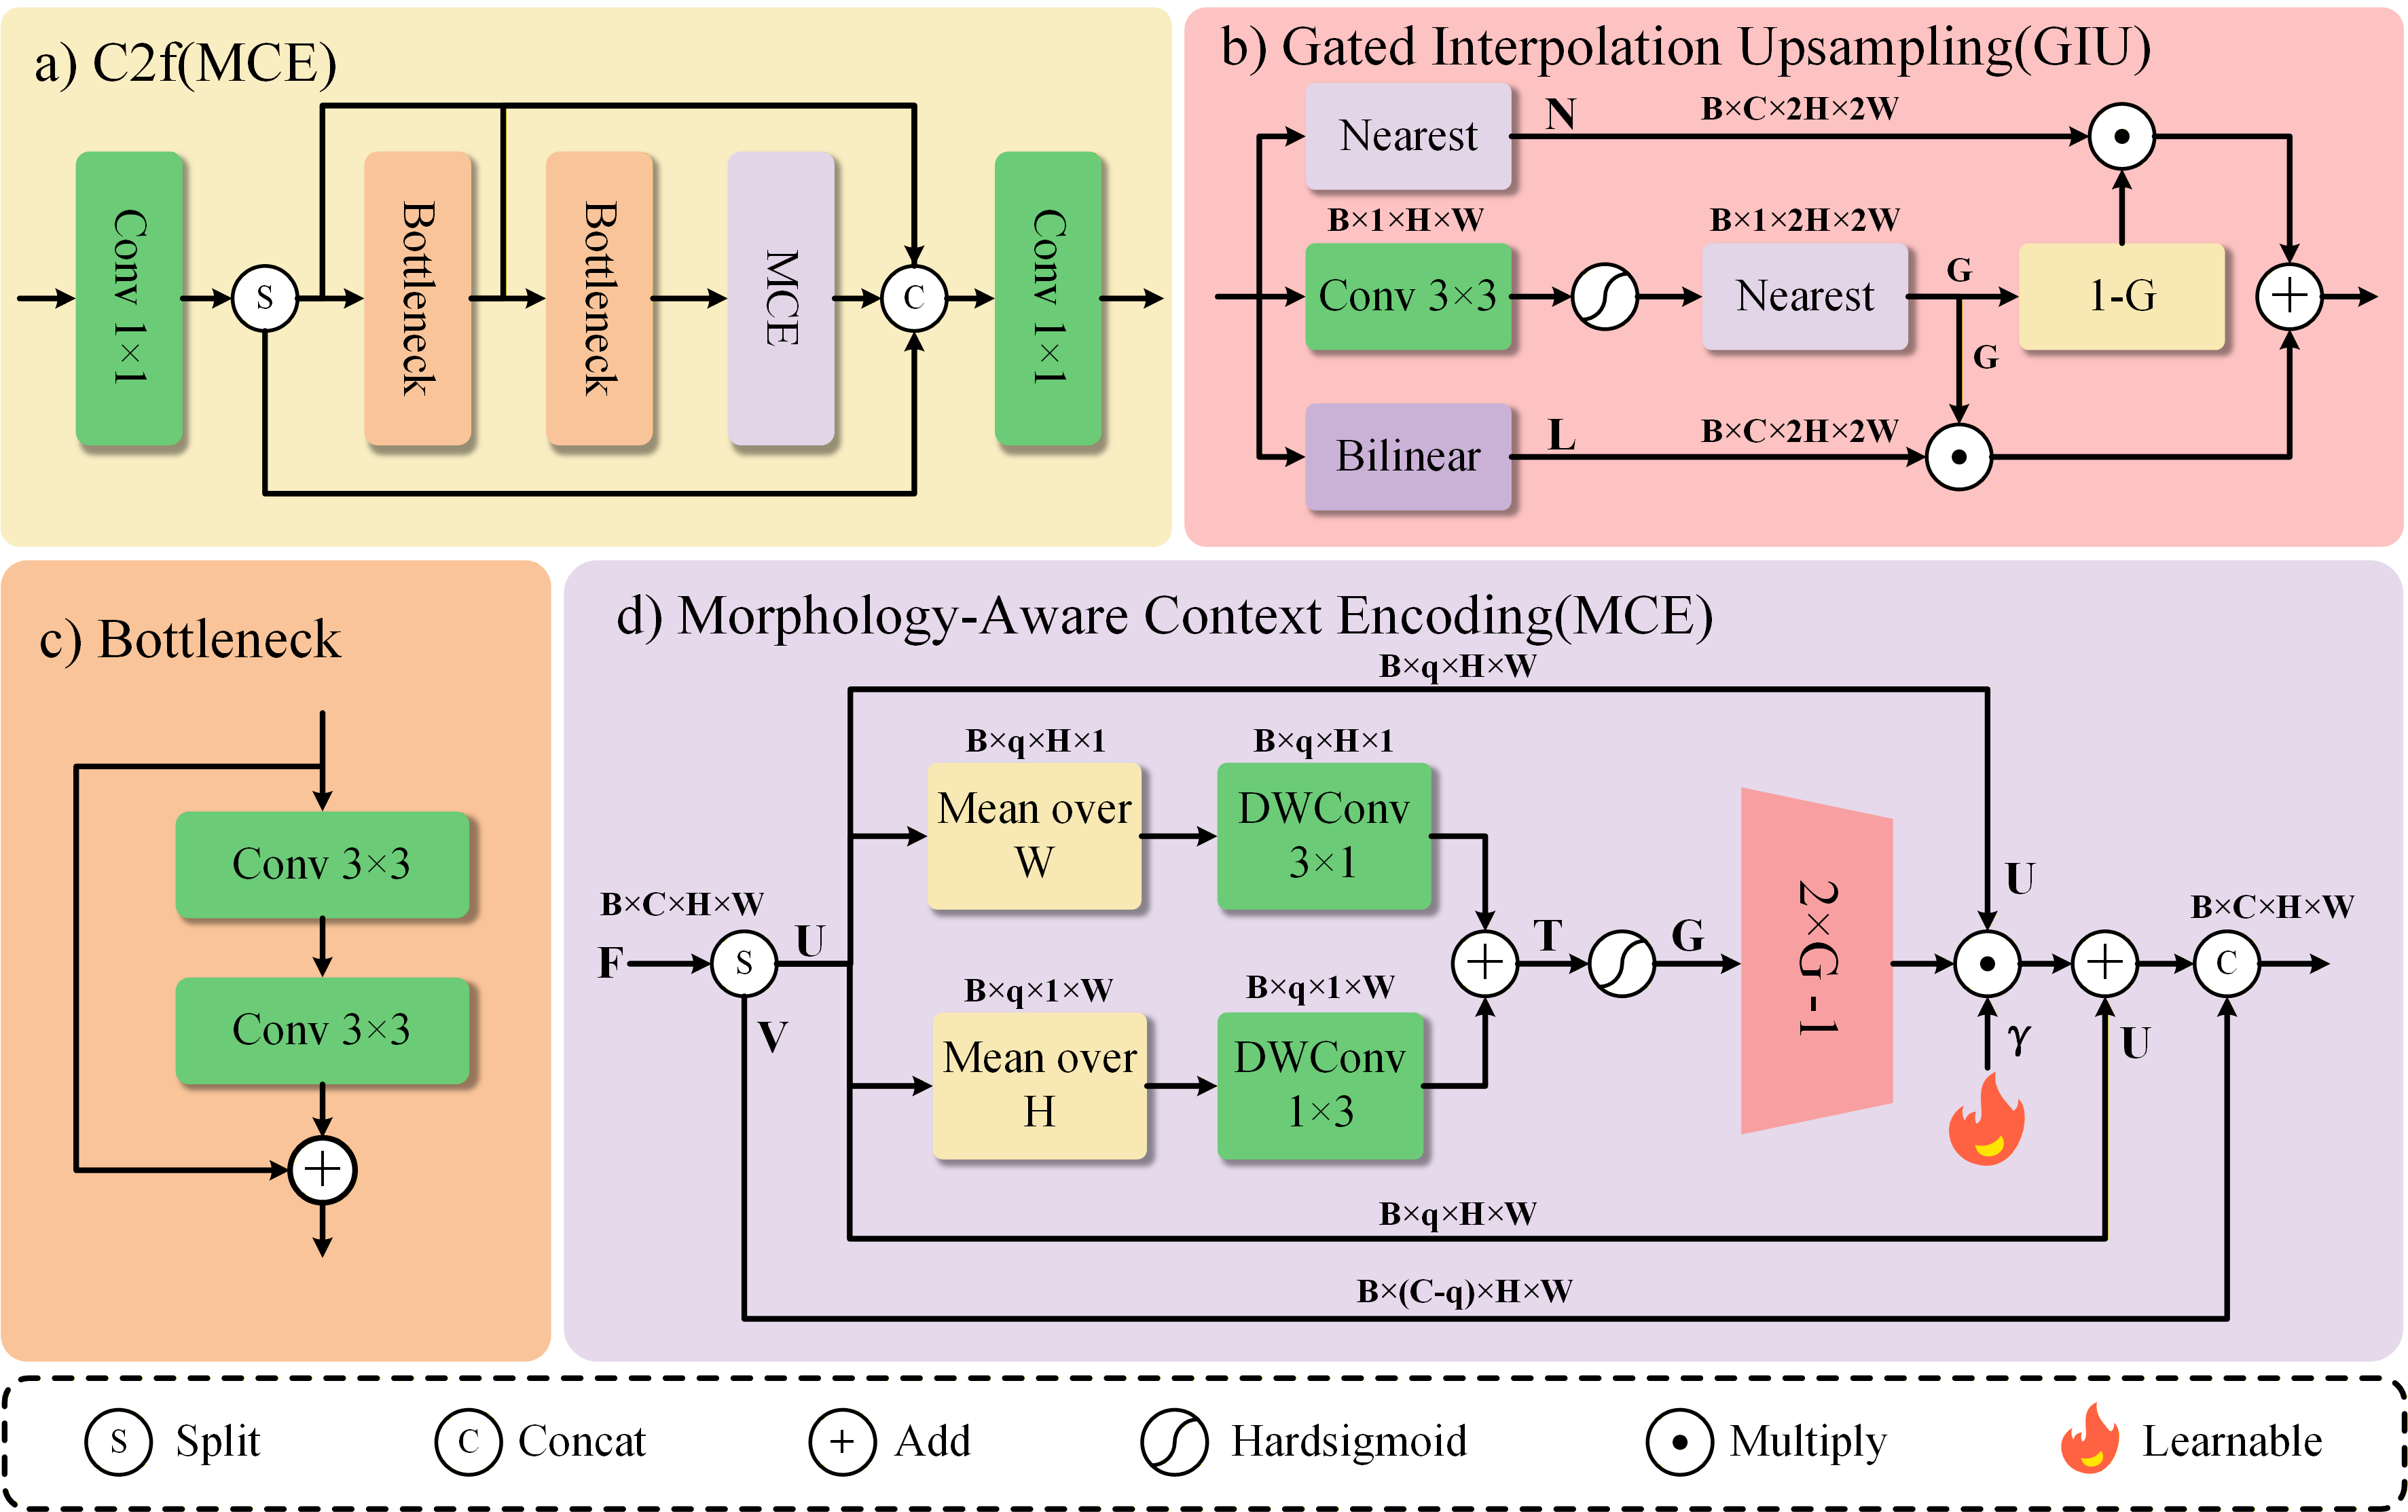
\includegraphics[width=0.9\textwidth]{MCE+GIU.png}
\caption{Structures of the proposed modules: (a) C2f block with MCE; (b) GIU with a spatial weight map shared across channels; (c) residual bottleneck retained in C2f; and (d) MCE with context modulation on one quarter of its input channels and an unchanged bypass for the remaining three quarters.}
\label{fig:modules}
\end{figure*}

\subsection{Gated Interpolation Upsampling}
Circular-knitting defects vary substantially in morphology and scale, from narrow horizontal and vertical patterns to small and large holes. Their feature representations therefore place different demands on spatial continuity, response concentration, and boundary extent. In the top-down feature pyramid, higher-level context must be reconstructed at a finer resolution before fusion with lateral features. Nearest-neighbor interpolation replicates responses within local regions, whereas bilinear interpolation combines neighboring responses to produce smoother spatial transitions. A fixed interpolation rule applies the same reconstruction behavior to all locations, limiting its adaptability to these diverse defect patterns. We develop GIU to adjust the balance between response replication and neighborhood smoothing according to the input features [Fig.~\ref{fig:modules}(b)]. To achieve this adaptation with a small computational overhead, GIU combines two parameter-free interpolation paths using a single spatial weight map predicted at low resolution and shared across channels. It reconstructs the higher-level context before fusion with shallow lateral features, which retain local texture and localization cues.

\emph{1) Two Fixed Interpolation Paths:}
For $X\in\mathbb{R}^{B\times C\times H\times W}$, nearest-neighbor and bilinear upsampling produce
\begin{align}
N &= \operatorname{Nearest}_{2}(X), \label{eq:giu-paths}\\
L &= \operatorname{Bilinear}_{2}(X), \label{eq:giu-bilinear}
\end{align}
where $N,L\in\mathbb{R}^{B\times C\times2H\times2W}$. Both operations use fixed interpolation weights and introduce no learnable parameters.

\emph{2) Shared Spatial Gate:}
A $3\times3$ convolution followed by Hardsigmoid predicts a low-resolution spatial weight map, which is then upsampled by nearest-neighbor interpolation:
\begin{align}
g &= \operatorname{HS}(\operatorname{Conv}_{3\times3}(X)), \label{eq:giu-gate-lowres}\\
G &= \operatorname{Nearest}_{2}(g), \label{eq:giu-gate}
\end{align}
where $\operatorname{Conv}_{3\times3}$ denotes a biased convolution with $C$ input channels, one output channel, and padding of 1, and $g\in[0,1]^{B\times1\times H\times W}$ is the low-resolution weight map. The map $G\in[0,1]^{B\times1\times2H\times2W}$ assigns a content-adaptive interpolation weight to each spatial location and is broadcast across feature channels. Predicting this map at $H\times W$ limits the spatial cost of the learned convolution, while channel sharing requires only one output weight per location.

\emph{3) Gated Reconstruction:}
The output $Y\in\mathbb{R}^{B\times C\times2H\times2W}$ is a convex combination:
\begin{equation}
Y=(1-G)\odot N+G\odot L.
\label{eq:giu-mixture}
\end{equation}
Small values of $G$ favor response replication, while larger values favor neighborhood smoothing. This spatially varying mixture allows the reconstruction behavior to adapt to local feature content associated with different defect morphologies and scales.
\begin{equation}
G_{\mathrm{init}}=0.05,\qquad Y_{\mathrm{init}}=0.95N+0.05L,
\label{eq:giu-initialization}
\end{equation}
so the module starts from a predominantly nearest-neighbor reconstruction, consistent with the baseline top-down pathway.

\section{Experimental Setup}
\label{sec:experimental-setup}
\subsection{Dataset}
The dataset was collected from a real circular-knitting production line and covers three defect categories: horizontal defects (\emph{row}), vertical defects (\emph{col}), and holes (\emph{hole}). It comprises 403 images with 468 annotated defect instances, divided into training, validation, and test sets of 282, 40, and 81 images, respectively, as summarized in Table~\ref{tab:data}.
\begin{table}[!htbp]
\caption{Image-level split and defect-instance counts in the real production-line dataset.}
\label{tab:data}
\centering
\footnotesize
\begin{tabular}{lrrrrr}
\toprule
Split & Images & Instances & Row & Col & Hole \\
\midrule
Train & 282 & 329 & 174 & 75 & 80 \\
Validation & 40 & 48 & 24 & 13 & 11 \\
Test & 81 & 91 & 60 & 12 & 19 \\
\bottomrule
\end{tabular}
\end{table}

\subsection{Implementation Details}
\label{sec:implementation}
\begin{table}[!htbp]
\caption{Implementation protocol covering training (Ultralytics) and deployment (edge device).}
\label{tab:implementation}
\centering
\footnotesize
\setlength{\tabcolsep}{3pt}
\renewcommand{\arraystretch}{1.08}
\begin{tabular}{@{}L{0.21\columnwidth}L{0.23\columnwidth}L{\dimexpr0.56\columnwidth-12pt\relax}@{}}
\toprule
Category & Parameter & Specification \\
\midrule
\multirow[t]{2}{0.21\columnwidth}{Training setup}
& Hardware & Intel i7-13700KF; NVIDIA RTX 3090 (24 GB) \\
& Software & Ubuntu 24.04, Python 3.10.20, PyTorch 2.4.1+cu124, and Ultralytics 8.4.140 \\
\midrule
\multirow[t]{3}{0.21\columnwidth}{Deployment setup}
& Hardware & Rockchip RK3566 \\
& System & Android 13 \\
& Quantization & INT8 \\
\midrule
Data protocol
& Input resolution & Fixed at $640\times640$ \\
\midrule
\multirow[t]{4}{0.21\columnwidth}{Training dynamics}
& Batch & 16  \\
& Maximum epochs & 300 \\
& Patience & 80 epochs \\
& Optimizer & AdamW \\
\bottomrule
\end{tabular}
\renewcommand{\arraystretch}{1.0}
\end{table}

% Queue wide comparison floats before the metrics to keep results illustrations nearby.
\begin{table*}[!tbp]
\caption{Detector comparison on the test set. FPS denotes FP32 model-forward throughput on an RTX 3090 with batch size 1 and a $640\times640$ input. Bold and underlined values indicate the best and second-best results, respectively.}
\label{tab:comparison}
\centering
\small
\setlength{\tabcolsep}{6pt}
\renewcommand{\arraystretch}{1.06}
\begin{tabular*}{\textwidth}{@{\extracolsep{\fill}}lrrrrr}
\toprule
Model & Params (M) & FLOPs (G) & mAP50 (\%) & mAP50--95 (\%) & FPS \\
\midrule
YOLOv9t~\cite{wang2025yolov9} & \textbf{2.12} & 8.5 & 90.1 & 53.3 & 291 \\
YOLOv10n~\cite{wang2024yolov10} & 2.78 & 8.8 & 88.2 & 58.5 & \underline{524} \\
YOLO11n~\cite{ultralytics2023} & 2.62 & \underline{6.7} & 93.3 & 60.8 & 463 \\
YOLO12n~\cite{tian2025yolov12} & 2.60 & 7.6 & 89.0 & 56.8 & 326 \\
YOLO26n~\cite{ultralytics2023} & \underline{2.57} & \textbf{6.2} & 90.5 & 58.2 & 425 \\
RT-DETR-R18~\cite{zhao2024rtdetr} & 20.09 & 60.7 & 95.2 & \textbf{67.7} & 146 \\
DETR-R50~\cite{carion2020detr} & 41.28 & 77.3 & 96.4 & 53.6 & 101 \\
Deformable DETR-R50~\cite{zhu2021deformable} & 39.8 & 158.7 & \underline{96.8} & 64.3 & 49 \\
Faster R-CNN-R50~\cite{ren2015faster} & 41.1 & 181.5 & 96.1 & 64.7 & 66 \\
YOLOv8n (Baseline)~\cite{ultralytics2023} & 3.01 & 8.1 & 90.5 & 58.4 & \textbf{554} \\
\model & 3.02 & 8.2 & \textbf{97.2} & \underline{65.5} & 486 \\
\bottomrule
\end{tabular*}
\par\smallskip
\renewcommand{\arraystretch}{1.0}
\end{table*}

\begin{figure*}[!tbp]
\centering
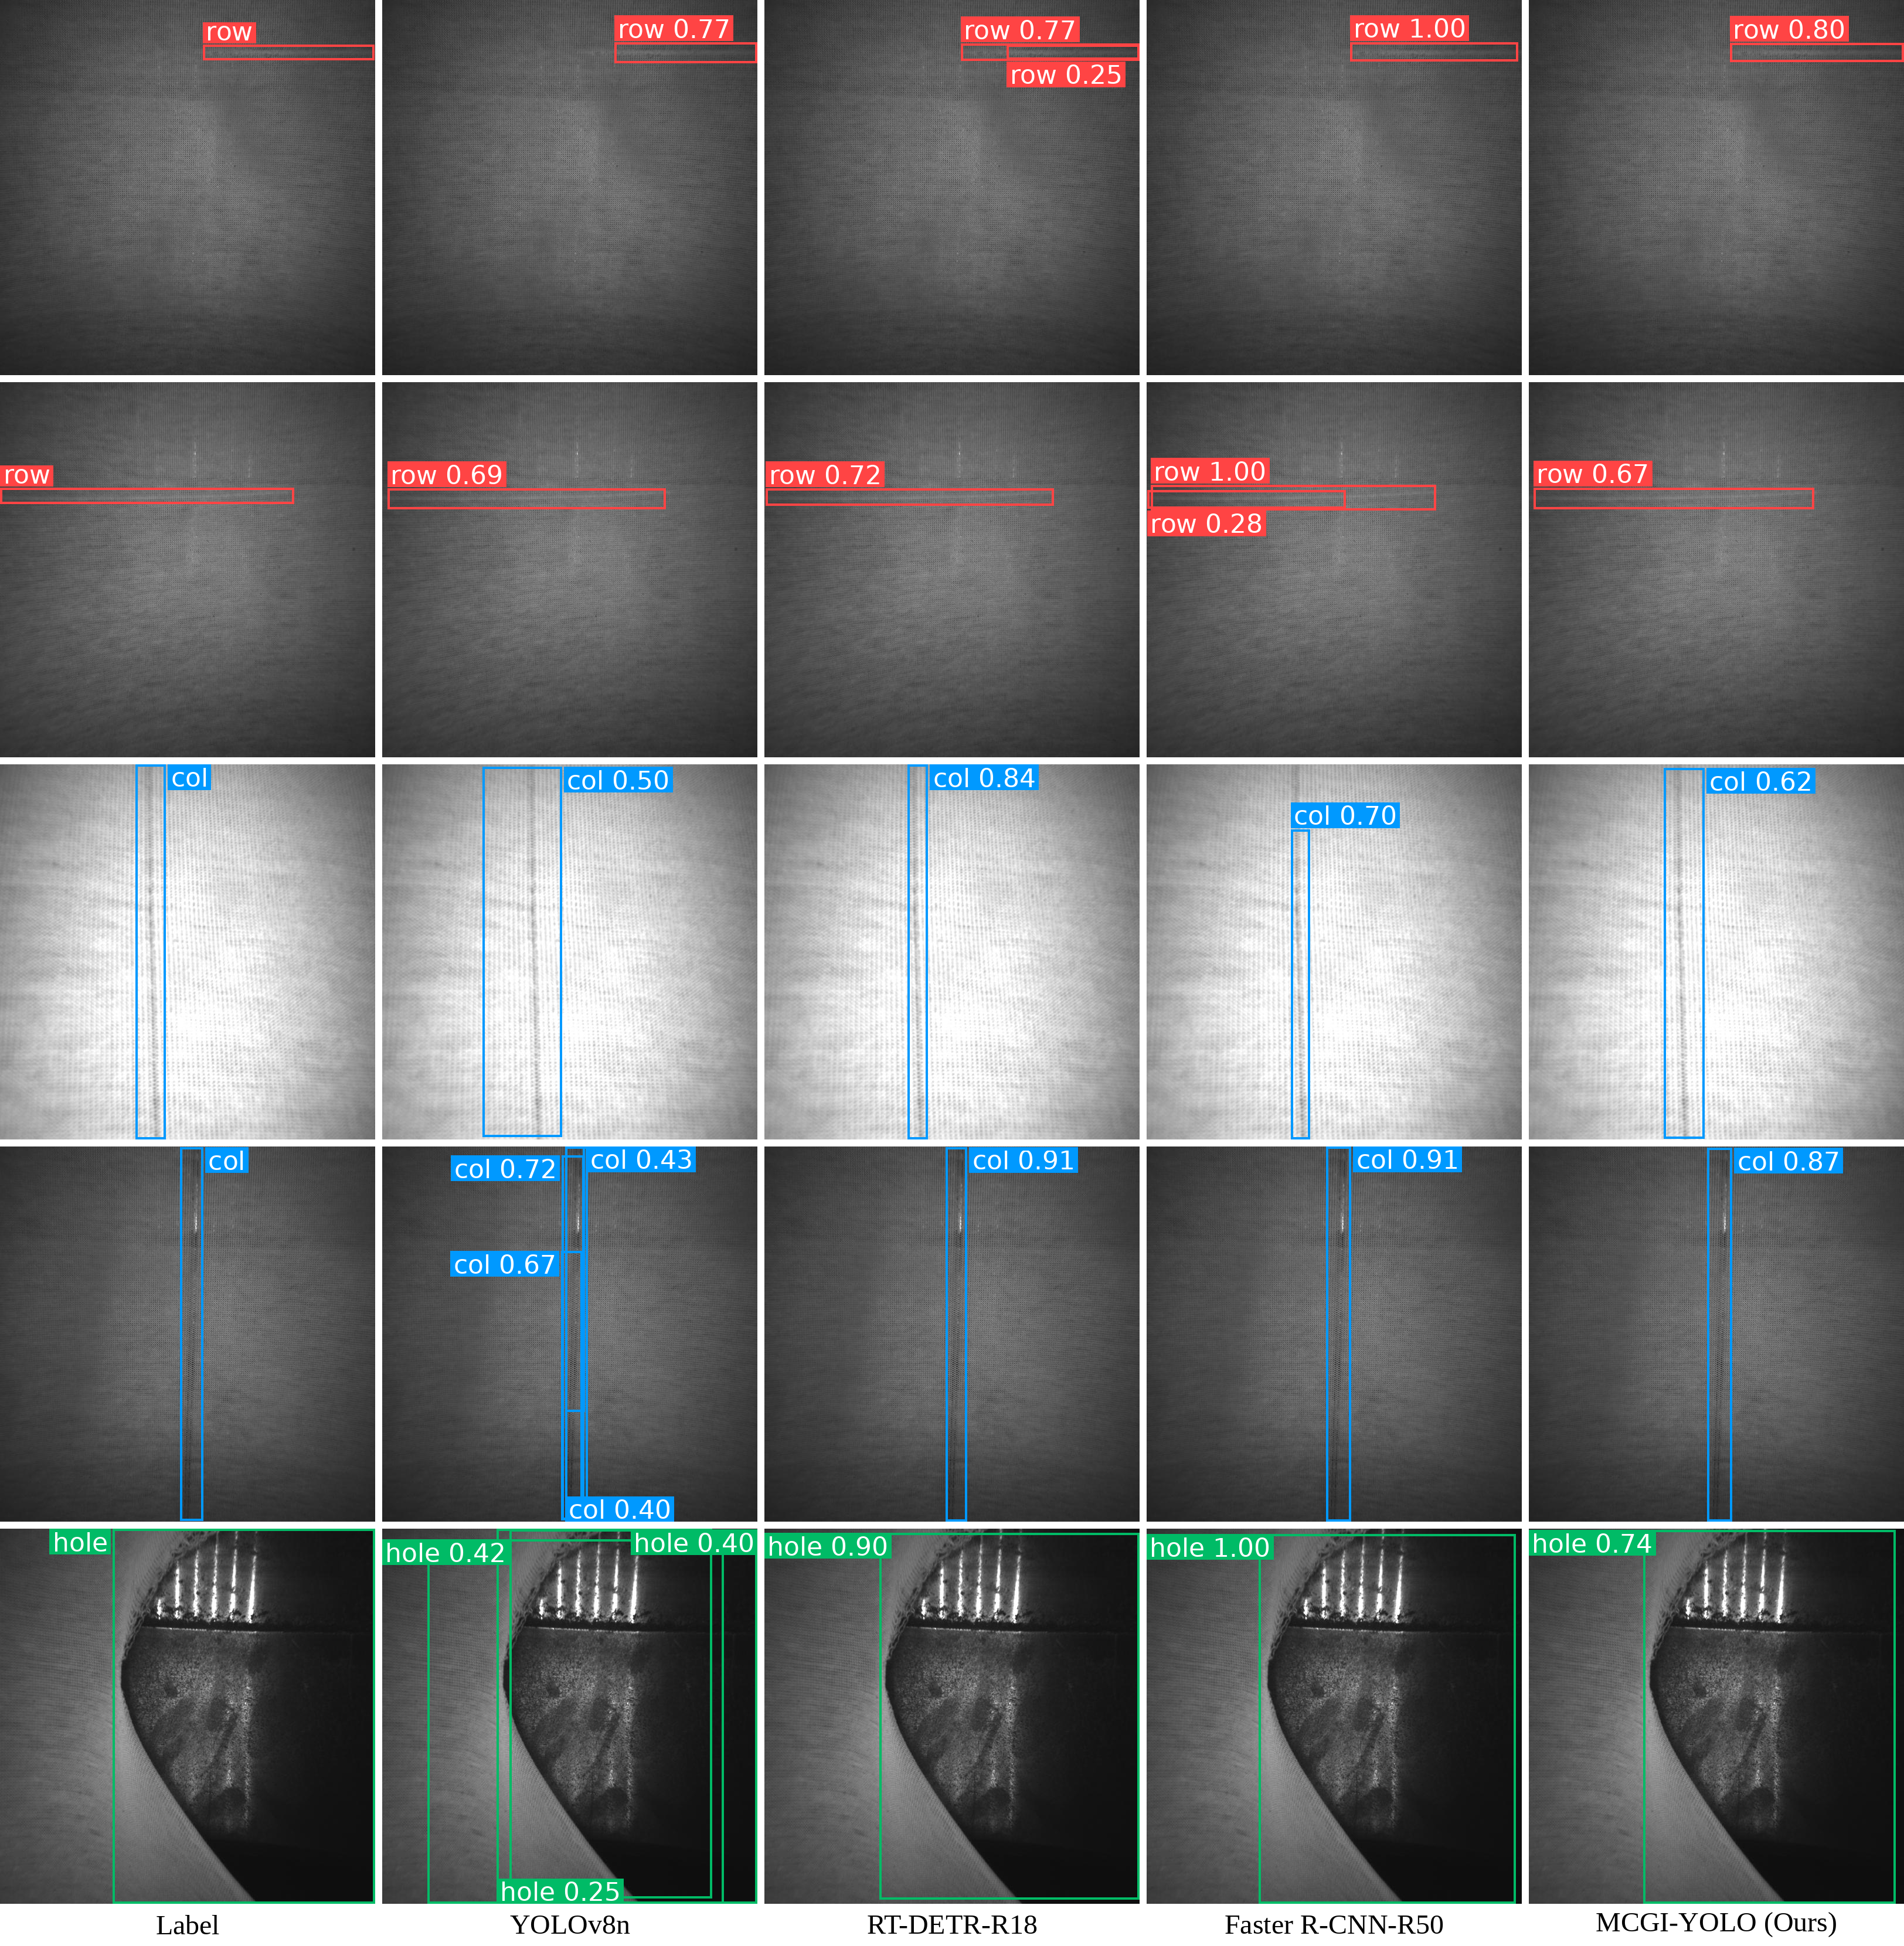
\includegraphics[width=0.86\textwidth]{compare.png}
\caption{Qualitative comparison of detection results across different methods. From left to right: ground-truth annotations (Label), YOLOv8n, RT-DETR-R18, Faster R-CNN-R50, and \model (Ours).}
\label{fig:qualitative}
\end{figure*}

Table~\ref{tab:implementation} summarizes the training and deployment settings. \model and its component-ablation variants share the same \texttt{yolov8n.pt} initialization as the YOLOv8n baseline, and all component comparisons use a common training protocol with matched random seeds. Other comparison models use available pretrained checkpoints from their respective implementations.

\subsection{Evaluation Metrics}
\label{sec:evaluation}
Intersection over union (IoU) measures the overlap between predicted and ground-truth bounding boxes as the ratio of their intersection area to their union area. Detection accuracy is evaluated using mAP50 and mAP50--95. Let $a_c(t)$ denote the average precision for class $c$ at IoU threshold $t$. The metrics are computed as
\begin{align}
\operatorname{mAP}_{50} &= \frac{1}{N_c}\sum_{c=1}^{N_c}a_c(0.50),
\label{eq:metrics}\displaybreak[1]\\
\operatorname{mAP}_{50:95} &= \frac{1}{10N_c}\sum_{c=1}^{N_c}\sum_{t\in T}a_c(t),
\label{eq:ap}
\end{align}
where $N_c=3$ and $T=\{0.50,0.55,\ldots,0.95\}$. Both metrics are reported as percentages, with improvements expressed in percentage points.

Model parameters and FLOPs are measured at $640\times640$ input resolution using each model's respective framework. For FPS comparison, all models are evaluated on an RTX 3090 with FP32 precision, batch size 1, and $640\times640$ inputs. This measurement is separate from the RK3566 deployment result.

\section{Results and Discussion}
\label{sec:results}
\subsection{Comparison With Other Detectors}
Table~\ref{tab:comparison} compares test-set accuracy, model complexity, and inference throughput. \model achieves the highest mAP50 of 97.2\% and the second-highest mAP50--95 of 65.5\%, improving over the YOLOv8n~\cite{ultralytics2023} baseline by 6.7 and 7.1 percentage points, respectively. This gain comes with only a marginal increase in parameters (3.01 M $\rightarrow$ 3.02 M) and FLOPs (8.1 G $\rightarrow$ 8.2 G), while throughput on the RTX 3090 decreases from 554 to 486 FPS. Among lightweight variants, YOLO11n~\cite{ultralytics2023} attains the next-best accuracy (93.3\% mAP50, 60.8\% mAP50--95); \model surpasses it by 3.9 and 4.7 points while running faster (486 vs.\ 463 FPS). YOLOv9t~\cite{wang2025yolov9}, YOLOv10n~\cite{wang2024yolov10}, YOLO12n~\cite{tian2025yolov12}, and YOLO26n~\cite{ultralytics2023} have fewer parameters or lower FLOPs but underperform on this test set, confirming that task-specific adaptation outperforms generic lightweight detectors. RT-DETR-R18~\cite{zhao2024rtdetr} leads in mAP50--95 (67.7\%) but requires 20.09 M parameters and 60.7 G FLOPs at 146 FPS. \model also outperforms DETR-R50~\cite{carion2020detr}, Deformable DETR-R50~\cite{zhu2021deformable}, and Faster R-CNN-R50~\cite{ren2015faster} on both mAP metrics with substantially lower cost, offering the best overall accuracy--efficiency tradeoff. Fig.~\ref{fig:qualitative} shows that \model produces fewer fragmented boxes and tighter localization on elongated defects and holes, consistent with the aggregate results.

\subsection{Component Ablation}
\label{sec:component-ablation}
\begin{table}[!htbp]
\caption{Component ablation of MCE and GIU.}
\label{tab:ablation}
\centering
\footnotesize
\setlength{\tabcolsep}{3pt}
\begin{tabular*}{\columnwidth}{@{\extracolsep{\fill}}lccrrrr@{}}
\toprule
Variant & MCE & GIU & Params(M) & FLOPs(G) & mAP50 & mAP50--95 \\
\midrule
YOLOv8n & -- & -- & 3.01 & 8.10 & 90.5 & 58.4 \\
+ MCE & \checkmark & -- & 3.01 & 8.2 & 93.9 & 63.6 \\
+ GIU & -- & \checkmark & 3.01 & 8.2 & 94.4 & 63.0 \\
\model & \checkmark & \checkmark & 3.02 & 8.2 & 97.2 & 65.5 \\
\bottomrule
\end{tabular*}
\end{table}

Table~\ref{tab:ablation} defines four configurations: the original YOLOv8n baseline, MCE alone, GIU alone, and their combination. The MCE-only model retains nearest-neighbor upsampling, while the GIU-only model retains the original backbone C2f blocks. On the test set, MCE alone achieves 93.9\% mAP50 and 63.6\% mAP50--95, improving over the baseline by 3.4 and 5.2 percentage points, respectively. GIU alone achieves 94.4\% and 63.0\%, corresponding to gains of 3.9 and 4.6 points. Combining the two modules yields 97.2\% mAP50 and 65.5\% mAP50--95, exceeding the best single-module result for each metric by 2.8 and 1.9 points. These results support the complementary benefits of morphology-aware context encoding and adaptive feature reconstruction. Feature visualizations in Fig.~\ref{fig:heatmaps} complement the numerical analysis by comparing responses at corresponding feature stages on the same images.



\subsection{Model Deployment and On-Device Performance}
\label{sec:deployment}
To deploy \model on the RK3566 edge device, the trained model is exported to ONNX with a fixed input size of $640\times$640 and then converted into an INT8 RKNN model using RKNN-Toolkit2 \cite{rockchiptoolkit2}. For $640\times$640 inputs, the deployed INT8 model achieves a measured inference throughput of 22 FPS on the RK3566. This throughput is 2.2 times the 10 FPS design target derived in Section~\ref{sec:coverage}, meeting the model-inference rate required for the specified machine speed and camera field of view.



\section{Conclusion}
\label{sec:conclusion}
This paper presents a dedicated defect detection and closed-loop control system for circular knitting machines, integrating image acquisition, SerDes transmission, edge inference, machine stopping, and cloud alerts. The lightweight \model combines MCE for elongated-defect morphology encoding with GIU for adaptive feature reconstruction. On the self-collected test set, it achieves 97.2\% mAP50 and 65.5\% mAP50--95, improving over YOLOv8n by 6.7 and 7.1 percentage points. INT8 deployment on the RK3566 achieves 22 FPS, exceeding the 10 FPS design target. Unlike generic object detection pipelines, our work jointly tailors both the hardware architecture and the detection algorithm to the morphology of knitting defects and the constraints of edge deployment, enabling real-time closed-loop control directly on the machine. By delivering a fully integrated and deployable system rather than an isolated algorithm, this work addresses a critical bottleneck in textile manufacturing—namely, the difficulty of translating detection performance into actionable, on-machine quality control. It offers the industry a ready-to-deploy reference for intelligent detection of circular knitting machines and, more broadly, demonstrates a reproducible pathway for deploying lightweight vision models on resource-constrained edge devices in industrial settings.

% Place the single-column feature visualization after the results text.
\begin{figure}[!hb]
\centering
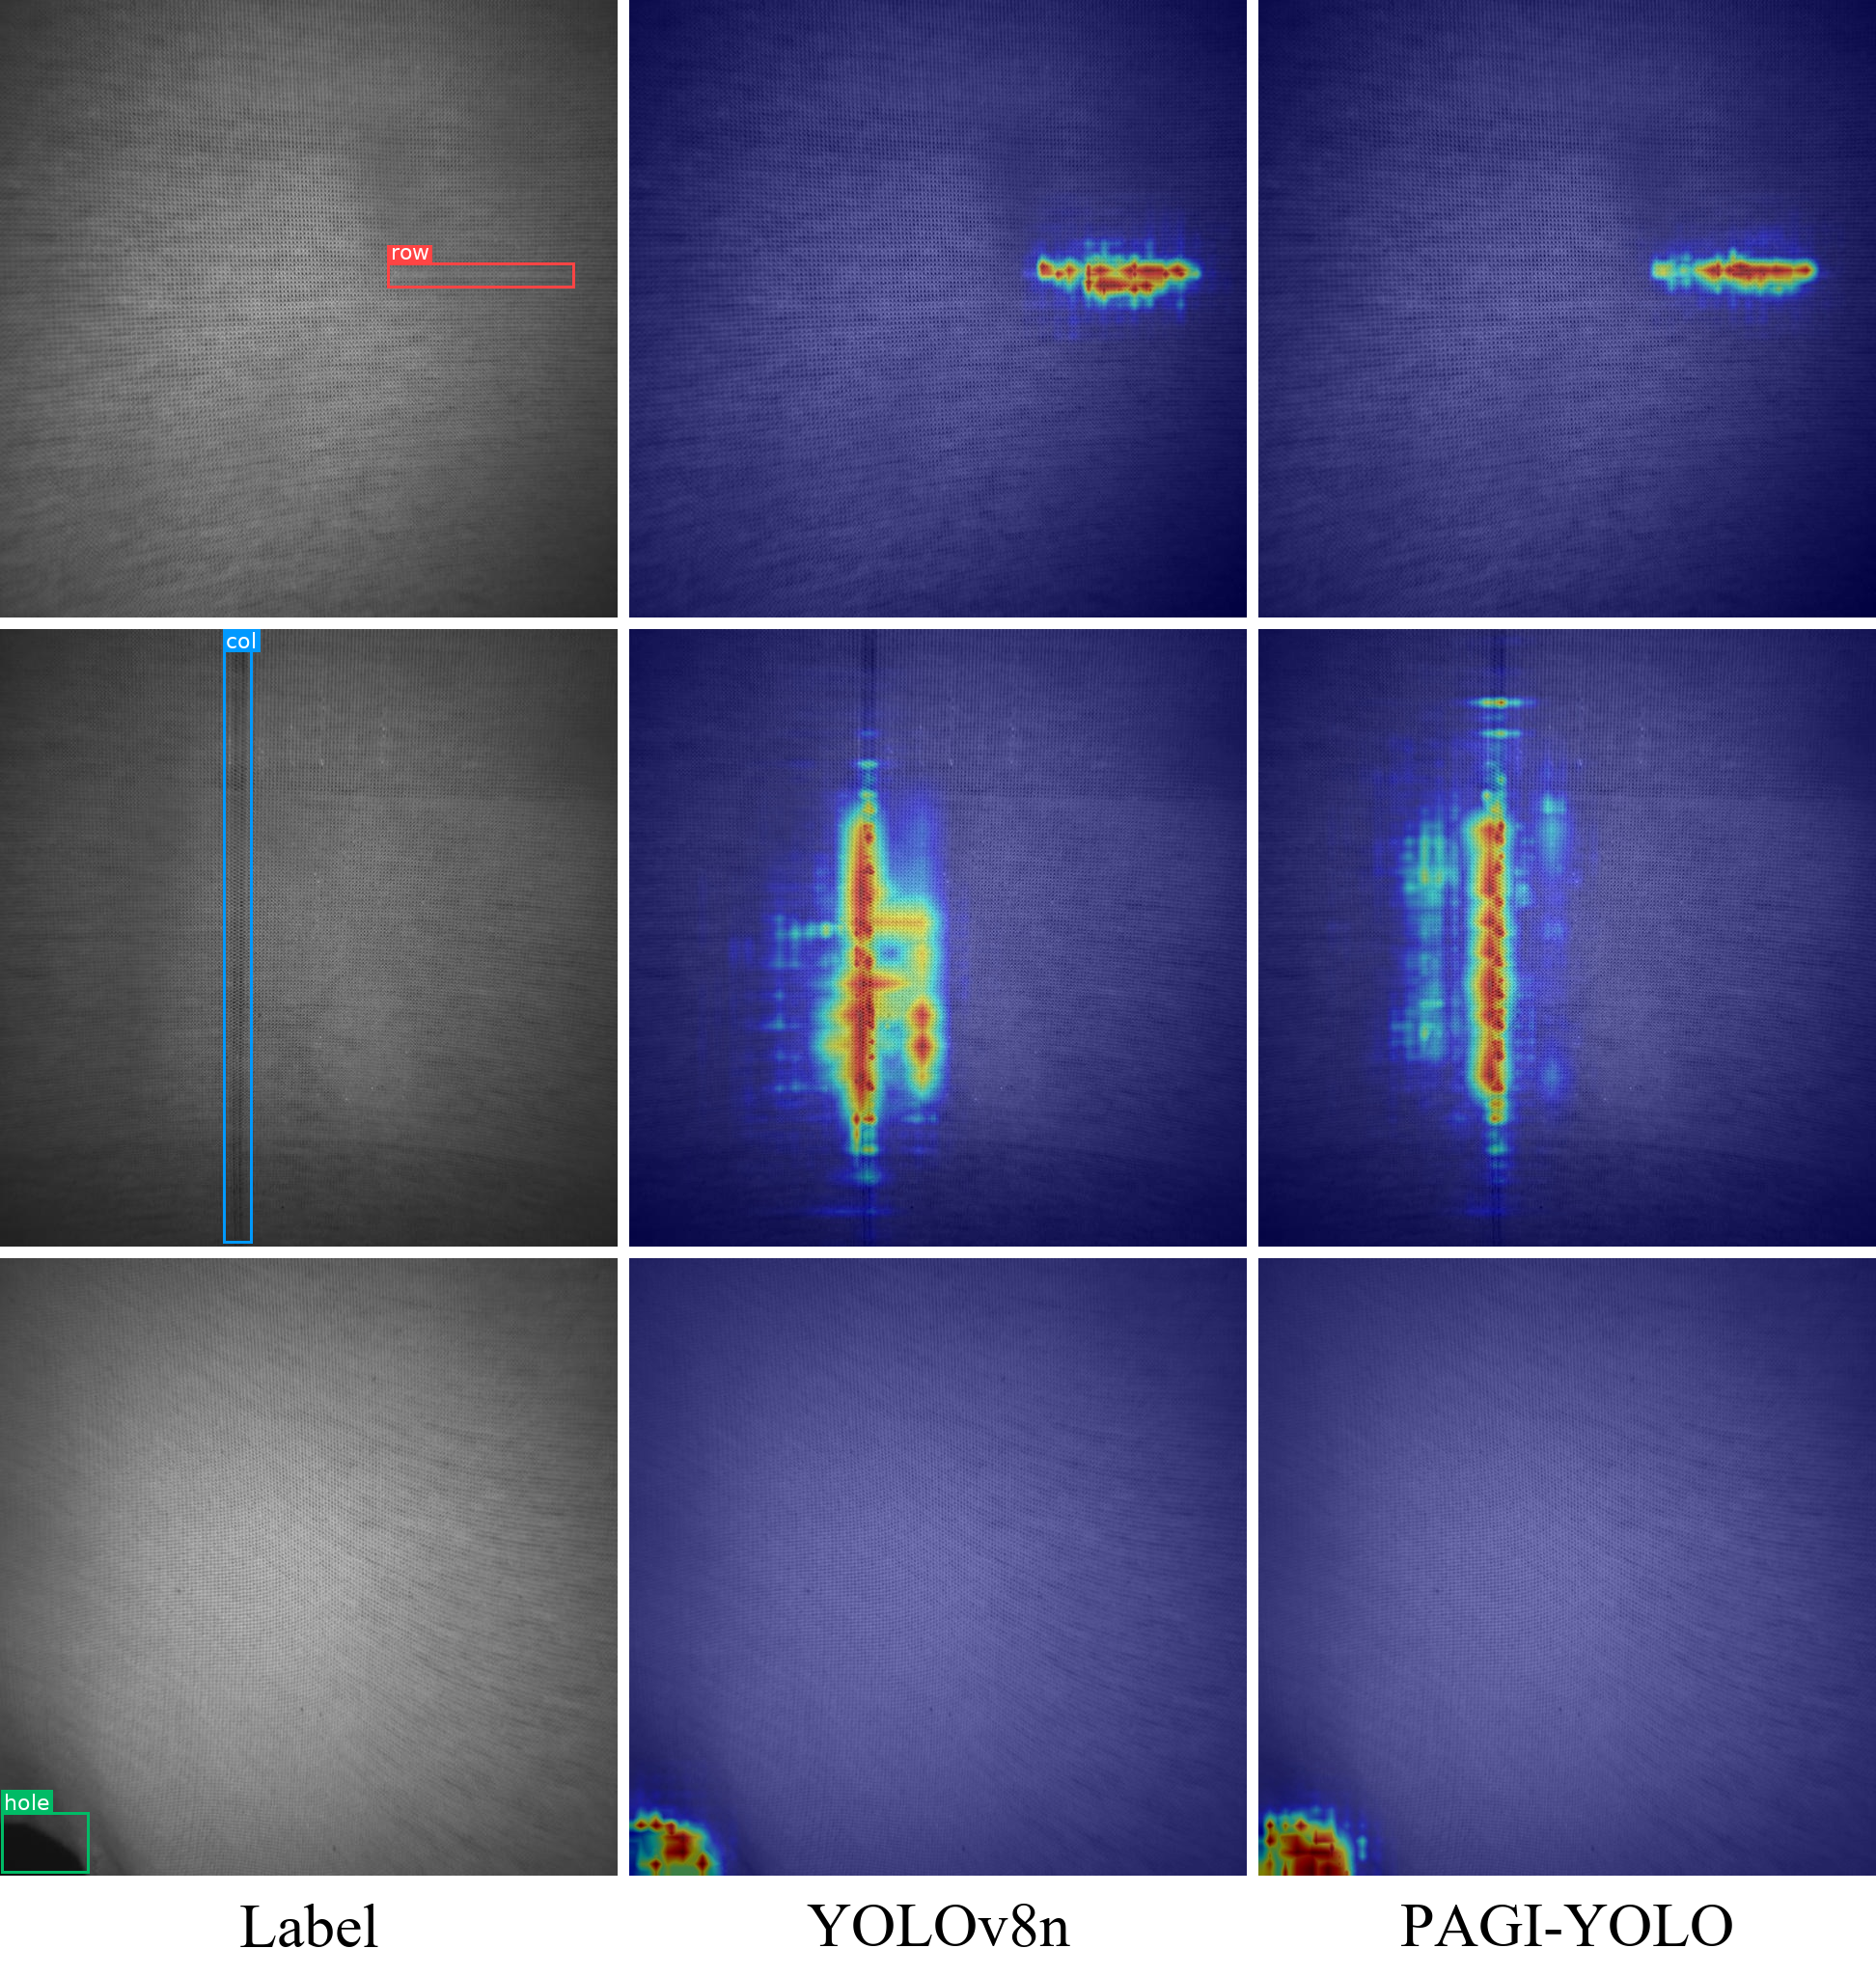
\includegraphics[width=\columnwidth]{heatmap_comparison.png}
\caption{Feature visualization of YOLOv8n and \model. From left to right: ground-truth annotations (Label), YOLOv8n, and \model.}
\label{fig:heatmaps}
\end{figure}

% Flush remaining results figures before the reference list.
\FloatBarrier
% Let remaining floats share pages with the following text.
\bibliographystyle{Bibliography/IEEEtranTIE}
\bibliography{references}

% Let biographies follow the completed references without forcing a new page.
% Author biographies follow the reference list in author order.
\begin{IEEEbiography}[{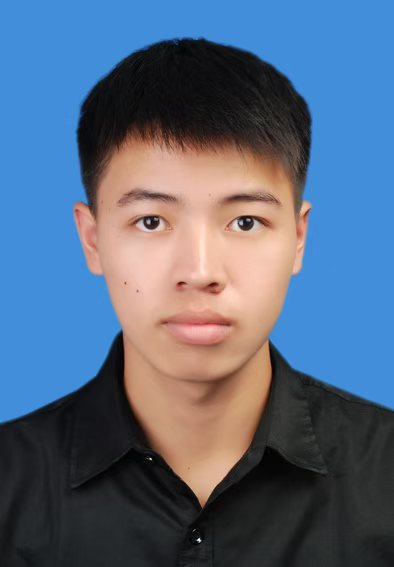
\includegraphics[width=1in,height=1.25in,clip,keepaspectratio]{a1.jpg}}]{Kangzhao Tan}
received the B.S. degree in computer science and technology from Guangzhou University, Guangzhou, China, in 2022. From 2022 to 2024, he worked as a cloud computing R\&D engineer with Sangfor Technologies Inc., Shenzhen, China. He is currently pursuing the M.S. degree in computer technology with the School of Computer Science, Guangdong University of Technology, Guangzhou, China. His research interests include deep learning, computer vision, and industrial defect detection.
\end{IEEEbiography}

\begin{IEEEbiography}[{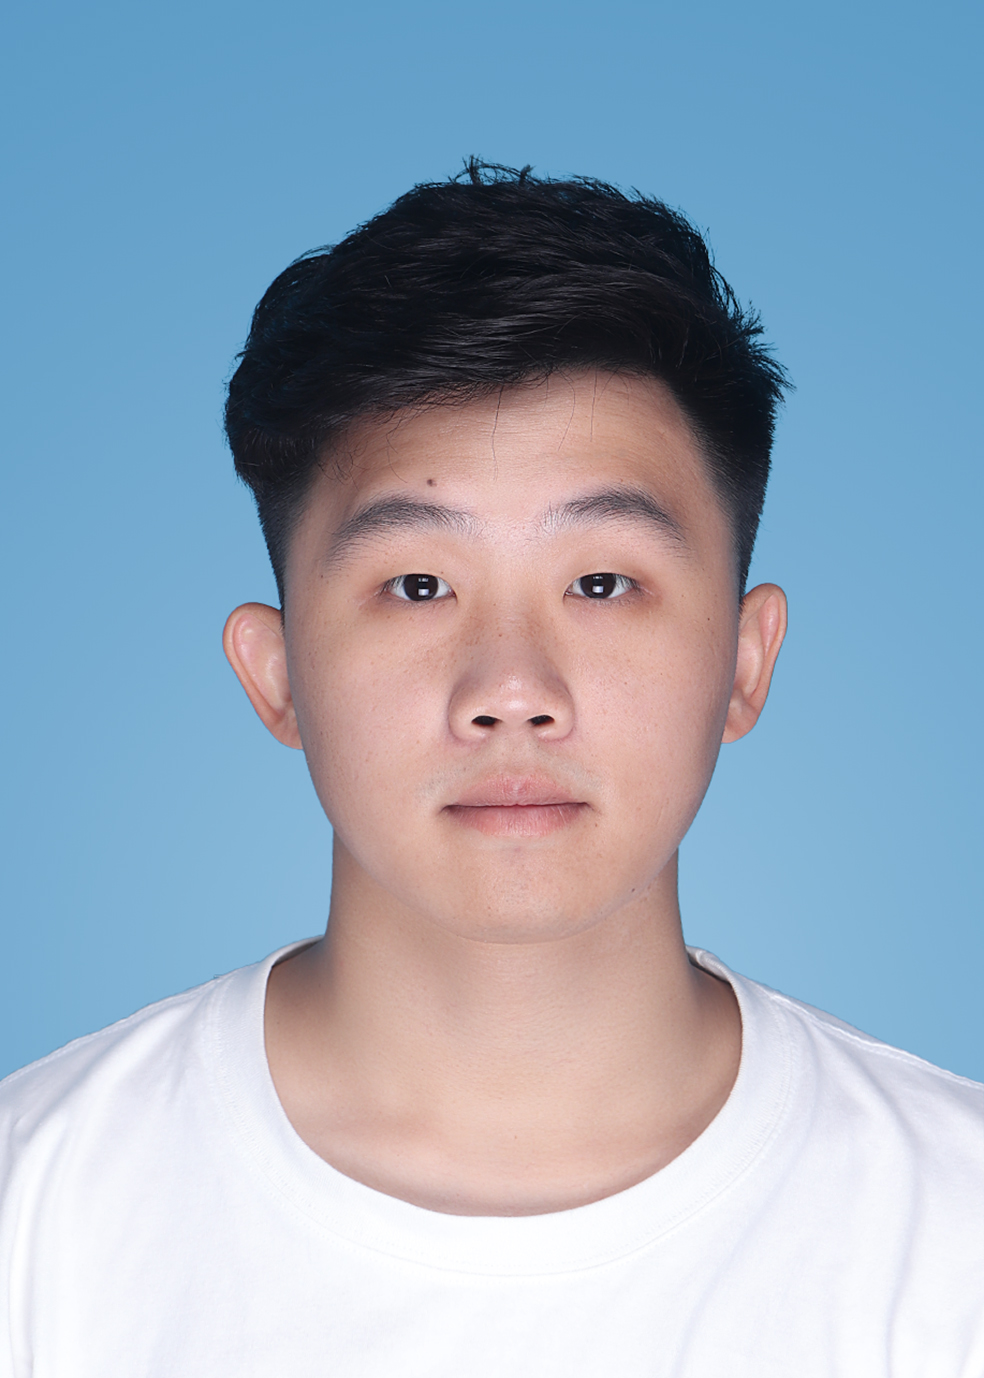
\includegraphics[width=1in,height=1.25in,clip,keepaspectratio]{a2.jpg}}]{Jiarui Zhang}
received the B.S. degree in electrical engineering and automation from Guangdong Polytechnic Normal University, Guangzhou, China, in 2021. He is currently pursuing the M.S. degree in software engineering with the School of Computer Science, Guangdong University of Technology, Guangzhou, China. His research interests include electronic circuit design and intelligent internet of things.
\end{IEEEbiography}

\begin{IEEEbiography}[{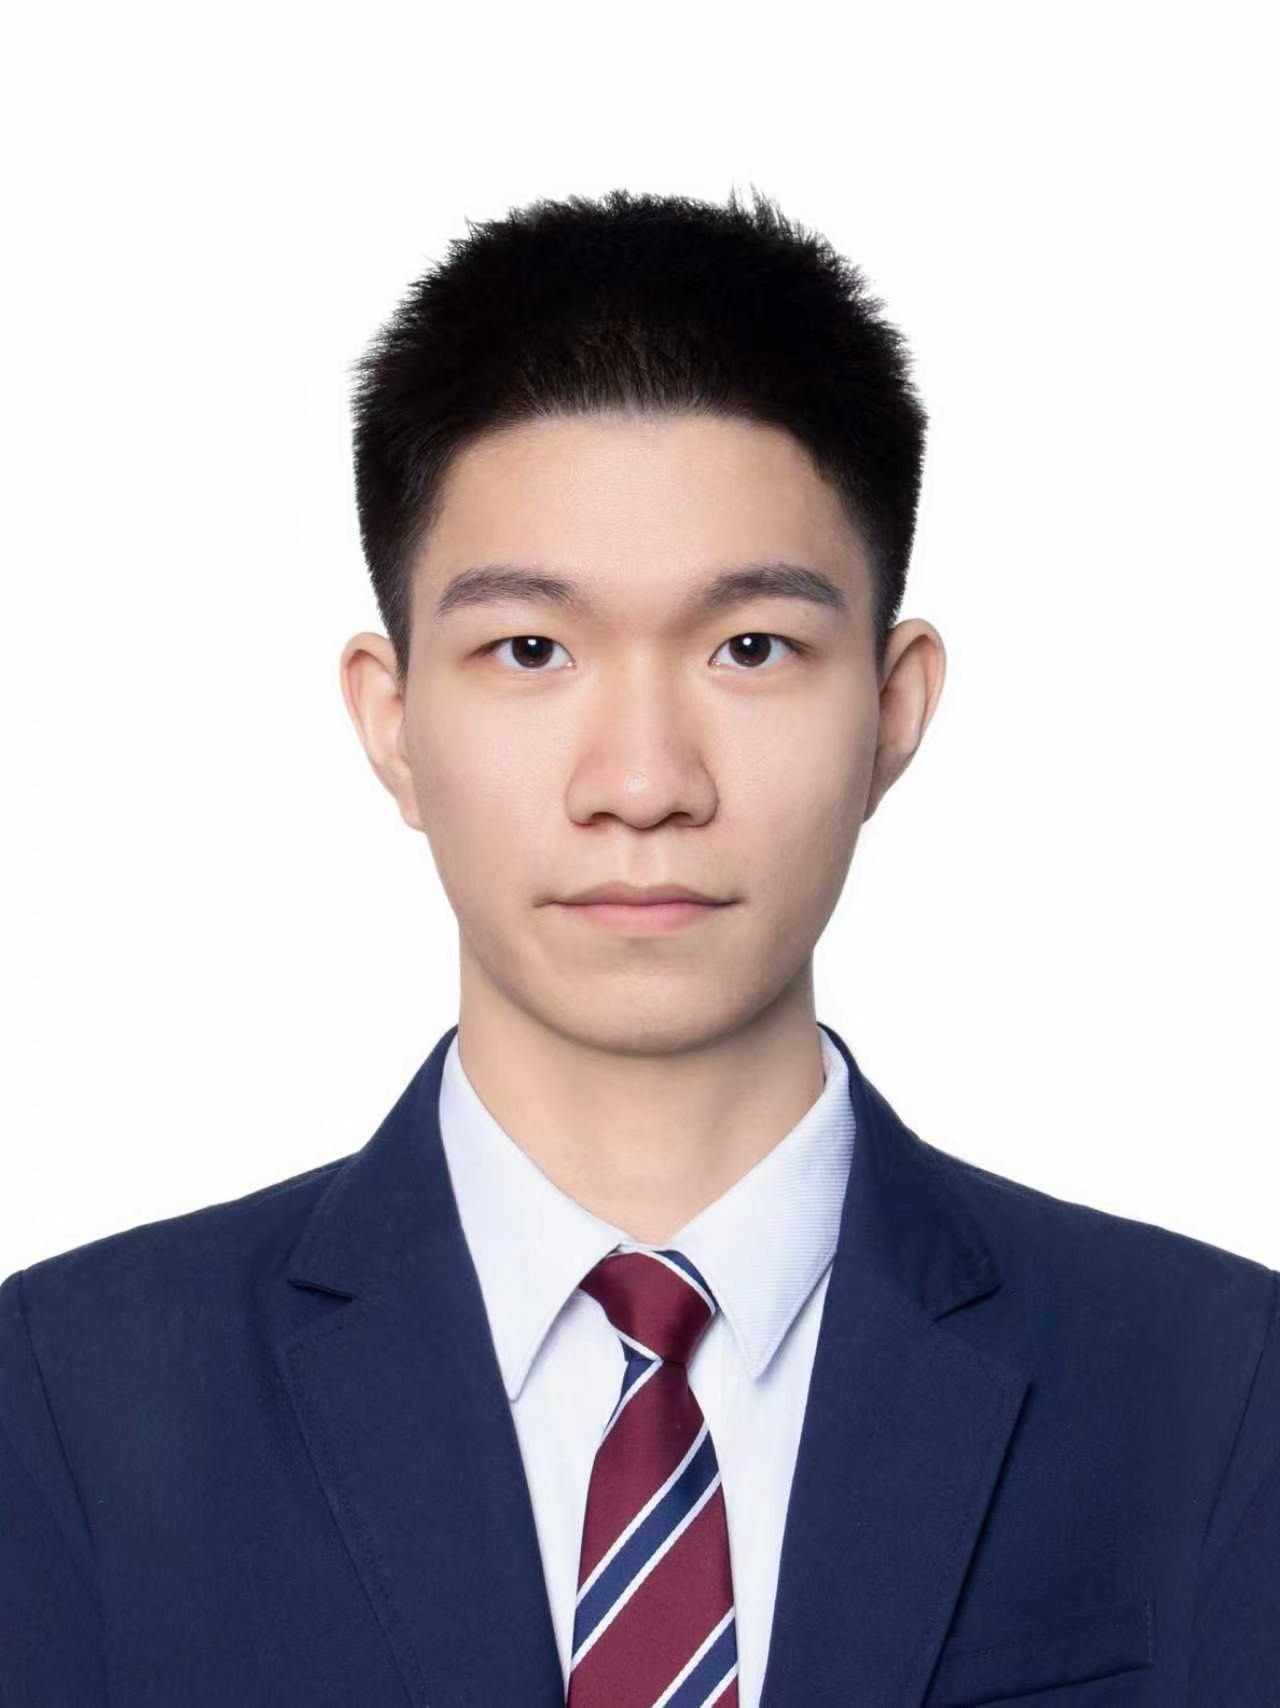
\includegraphics[width=1in,height=1.25in,clip,keepaspectratio]{a3.jpg}}]{Junjie Yu}
received the B.S. degree in computer science and technology from Hunan University of Finance and Economics, Changsha, China, in 2025. He is currently pursuing the M.S. degree in computer technology at Guangdong University of Technology, Guangzhou, China.
His current research interests include image processing and edge computing.
\end{IEEEbiography}

\begin{IEEEbiography}[{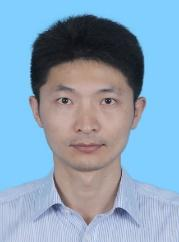
\includegraphics[width=1in,height=1.25in,clip,keepaspectratio]{a4.jpg}}]{Heng Wu}
received the B.S. degree in electronic and information engineering from Wuhan University of Science and Technology, Wuhan, China, in 2009, and the M.S. degree in optics and the Ph.D. degree in mechanical manufacturing and automation from South China University of Technology, Guangzhou, China, in 2012 and 2017, respectively.

He is currently an associate professor with the School of Automation, Guangdong University of Technology. His research interests include optical imaging, optical measurement, machine vision, and image processing.
\end{IEEEbiography}

\begin{IEEEbiography}[{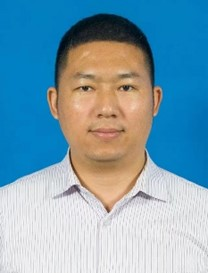
\includegraphics[width=1in,height=1.25in,clip,keepaspectratio]{a5.jpg}}]{Jing Lin}
received the B.S. degree in computer science and technology and the M.S. degree in software engineering from Guangdong University of Technology, Guangzhou, China, in 2003 and 2006, respectively.

Since graduation, he has served as an assistant engineer, engineer, and senior engineer. He is currently a senior engineer with the Classroom Management Center, Guangdong University of Technology. His current research interests include information system project management, system informatization, and the intelligent Internet of Things.
\end{IEEEbiography}

\begin{IEEEbiography}[{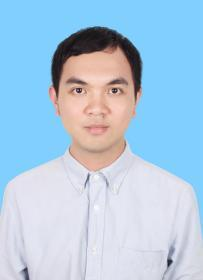
\includegraphics[width=1in,height=1.25in,clip,keepaspectratio]{a6.jpg}}]{Chunhua He}
received the B.S. degree in microelectronics from Sun Yat-sen University, Guangzhou, China, in 2010, and the M.S. and Ph.D. degrees in microelectronics from Peking University, Beijing, China, in 2013 and 2018, respectively.

From 2013 to 2017, he was an engineer with the No. 5 Electronics Research Institute, Ministry of Industry and Information Technology, Guangzhou, China. From 2017 to 2019, he was an engineer with Midea Group, Foshan, China. From 2019 to 2021, he was a senior engineer with Guangzhou 37 Degree Smart Home Co., Ltd., Guangzhou, China. He joined the School of Computer Science, Guangdong University of Technology, Guangzhou, China, in 2021, where he is currently a professor. His current research interests include the design and application of MEMS sensors and artificial intelligence algorithms.
\end{IEEEbiography}

\end{document}
